 \documentclass{beamer}
%
% Choose how your presentation looks.
% For more themes, color themes and font themes, see:
% http://deic.uab.es/~iblanes/beamer_gallery/index_by_theme.html
%
\mode<presentation>
{
  \usetheme{Madrid}      % or try Darmstadt, Madrid, Warsaw, ...
  \usecolortheme{seahorse} % or try albatross, beaver, crane, ...
  \usefonttheme{serif}  % or try serif, structurebold, ...
  \setbeamertemplate{navigation symbols}{}
  \setbeamertemplate{caption}[numbered]
  \usepackage{amsmath}
  \usepackage{tcolorbox}
  \usepackage[export]{adjustbox}
  \tcbuselibrary{most}
  \usepackage{arydshln}
  \usepackage{tikz}
  \usetikzlibrary{plotmarks}
  \usepackage{pgfplots}
  \usepackage{cancel}
 %\usepackage{enumitem}
%\usepackage{enumerate}
  %\usepackage[shortlabels]{enumitem}
} 


\definecolor{myblue}{RGB}{65,105,225} 
\definecolor{myorange}{RGB}{250,190,0}

\setbeamercolor{structure}{fg=white,bg=myorange}
\setbeamercolor*{palette primary}{fg=myblue,bg=myorange}
\setbeamercolor*{palette secondary}{fg=white,bg=myblue}
\setbeamercolor*{palette tertiary}{bg=myblue,fg=white}
\setbeamercolor*{palette quaternary}{fg=white,bg=myorange!50}

\setbeamercolor{frametitle}{fg=black!90!myblue}

\setbeamercolor{section in head/foot}{fg=white,bg=myblue}
\setbeamercolor{author in head/foot}{fg=black,bg=myorange}
\setbeamercolor{title in head/foot}{fg=white,bg=myblue}

\setbeamertemplate{navigation symbols}{}

\setbeamertemplate{itemize/enumerate body begin}{\large}
\setbeamertemplate{itemize/enumerate subbody begin}{\large}
\setbeamertemplate{itemize/enumerate subsubbody begin}{\large}



\defbeamertemplate*{headline}{mytheme}
{%
  \begin{beamercolorbox}[ht=2.25ex,dp=3.75ex]{section in head/foot}
    \insertnavigation{\paperwidth}
  \end{beamercolorbox}%
}%

\defbeamertemplate*{footline}{mytheme}
{
  \leavevmode%
  \hbox{%
  \begin{beamercolorbox}[wd=.5\paperwidth,ht=2.25ex,dp=1ex,right]{author in head/foot}%
    \usebeamerfont{author in head/foot}\insertshortauthor\hspace*{2em}
  \end{beamercolorbox}%
  \begin{beamercolorbox}[wd=.5\paperwidth,ht=2.25ex,dp=1ex,left]{title in head/foot}%
    \usebeamerfont{title in head/foot}\hspace*{2em}\insertshortsubtitle\hspace*{2em}
    \insertframenumber{} / \inserttotalframenumber
  \end{beamercolorbox}}%
  \vskip0pt%
}

\usepackage[english]{babel}
%\usepackage[utf8x]{inputenc}
\usepackage{xcolor}
\usepackage{listings}
\usepackage{pgf}  
\usepackage{textpos}
\usepackage{tabulary}
\usepackage{booktabs}
\usepackage{systeme, mathtools}
\usepackage{scrextend}
\usepackage{hyperref}
\usepackage{setspace}
\usepackage{rotating}
\lstset
{
    language=[LaTeX]TeX,
    breaklines=true,
    basicstyle=\tt\scriptsize,
    %commentstyle=\color{green}
    keywordstyle=\color{blue},
    %stringstyle=\color{black}
    identifierstyle=\color{magenta},
}
\newcommand{\bftt}[1]{\textbf{\texttt{#1}}}
%\newcommand{\comment}[1]{{\color[HTML]{008080}\textit{\textbf{\texttt{#1}}}}}
\newcommand{\cmd}[1]{{\color[HTML]{008000}\bftt{#1}}}
\newcommand{\bs}{\char`\\}
\newcommand{\cmdbs}[1]{\cmd{\bs#1}}
\newcommand{\lcb}{\char '173}
\newcommand{\rcb}{\char '175}
\newcommand{\cmdbegin}[1]{\cmdbs{begin\lcb}\bftt{#1}\cmd{\rcb}}
\newcommand{\cmdend}[1]{\cmdbs{end\lcb}\bftt{#1}\cmd{\rcb}}

\newcommand{\wllogo}{\textbf{Overleaf}}

% this is where the example source files are loaded from
% do not include a trailing slash
\newcommand{\fileuri}{https://raw.githubusercontent.com/GiancarloSucci/UniBo.IDSEPC.A2022/main/A2022.IDSEPCLaTeX/}


\usepackage{stackengine}
\def\Ruble{\stackengine{.67ex}{%
  \stackengine{.48ex}{\textsf{P}}{\rule{.8ex}{.12ex}\kern.6ex}{O}{r}{F}{F}{L}%
  }{\rule{.8ex}{.12ex}\kern.6ex}{O}{r}{F}{F}{L}\kern-.1ex}
\DeclareMathOperator*{\argmax}{argmax}



%----------------------------------------------------------------------------------------
%	TITLE PAGE
%----------------------------------------------------------------------------------------
\title[L01]{Artificial Intelligence, Blockchain, e Criptovalute nello Sviluppo Software \newline\newline
Lezioni 13 e 14: Inferences, Non Parametric Approaches, and Logistic Regression} % The short title appears at the bottom of every slide, the full title is only on the title page

\author[{\tiny Giancarlo Succi }]{Giancarlo Succi\\\\ Dipartimento di Informatica -- Scienza e Ingegneria\\Universit\`{a} di Bologna\\
\bftt{g.succi@unibo.it}
} % Your name
\institute[unibo] % Your institution as it will appear on the bottom of every slide, may be shorthand to save space


\date{} % Date, can be changed to a custom date

\setbeamertemplate{navigation symbols}{}
\AtBeginSection[]
{
        \begin{frame}<beamer>{Outline}
                \tableofcontents[currentsection]
        \end{frame}
}
\begin{document}
\begin{frame}
\titlepage % Print the title page as the first slide

\end{frame}

%=============================================

\addtobeamertemplate{frametitle}{}{%
\begin{textblock*}{10mm}(-0.01mm,-0.95cm)

\includegraphics[width=0.9cm]{unibo-logo.png}
\end{textblock*}}

%=============================================
\begin{frame}
{\centerline{Content}}

\begin{itemize}
\item More on the correlation coefficient
\item Non parametric correlations
\item Logistic regression
\end{itemize}
\end{frame}

%=============================================

%=============================================
%------------------------------------------------
\begin{frame}
{\centerline{Part 1}}

\begin{center}
\Huge More on the correlation coefficient
\end{center}
\end{frame}

%----------------------------------------------------------------------------------------

\begin{frame}
{\centerline{Status}}

\begin{itemize}
\item Now we know that the means of samples of a population tend to be distributed normally.
\item This is an essential assumption to perform several numeric operations, like Montecarlo simulations, Bootstrap, etc.
\item We would like now to understand the distribution of the Pearson momentum correlation coefficient of the sample
\item Moreover, we have an open infinite issue on what to do if the data is NOT on a ratio scale
\end{itemize}


\end{frame}


\begin{frame}
{\centerline{Modeling with linear models (1/2)}}
Linear regression is dependent on 4 hypothesis:
\begin{enumerate}
\item Normality\\
The dependent variable is normally distributed at each value of the independent variables. \\
\textit{How to check:} histogram of standardized residuals, Q-Q plot
\item Homoscedasticity\\
The variability of the standardized residuals is constant and does not depend on dependent variable.\\
\textit{How to check:} plotting the residuals over the mean value of dependent variable
\end{enumerate}

\end{frame}
%----------------------------------------------------------------------------------------
%------------------------------------------------
%----------------------------------------------------------------------------------------
%------------------------------------------------
\begin{frame}
{\centerline{Modeling with linear models (2/2)}}
\begin{enumerate}
\item Independence of error\\
Each value of the residual does not depend in some way from the preceding value.\\
\textit{How to check:} Durbin-Watson statistic
\item Linearity\\
There is linear dependency between regressors and response\\
\textit{How to check:} linear correlation coefficient
\end{enumerate}

\end{frame}

\begin{frame}
{\centerline{Is the correlation enough for predicting?}}

\begin{itemize}
\item The size of an acceptable correlation depends on the context
\item A key question is what is the additional explanation that I get from analysing $X$ vs just using $Y$
\item The following diagram for instance shows how the 95\% confidence interval is reduced for increasing values of the correlation
\end{itemize}
\vspace*{-0.5cm}
\begin{center}
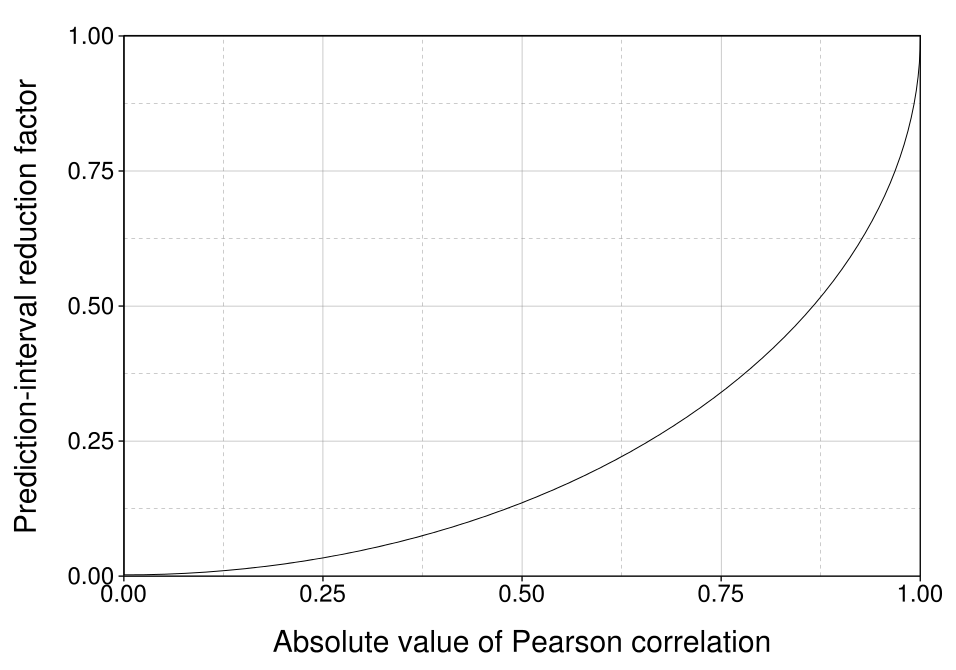
\includegraphics[width=5.5cm]{P2023.AIBCCSS.InferenceAndLogisticRegression/956px-Pearson_correlation_and_prediction_intervals.png}
\end{center} 
\vspace*{-0.5cm}
\textit{\tiny
\vspace{-\baselineskip}
Source with modifications: \url{https://en.wikipedia.org/wiki/Pearson_correlation_coefficient}}

\end{frame}


\begin{frame}
{\centerline{Spurious correlations. Why?}}


\textbf{Comparing "Apples and Oranges"}

Y axis scales that measure different values may show similar curves that shouldn’t be paired. This becomes pernicious when the values appear to be related but aren’t.

\textbf{Example. }

\begin{center}
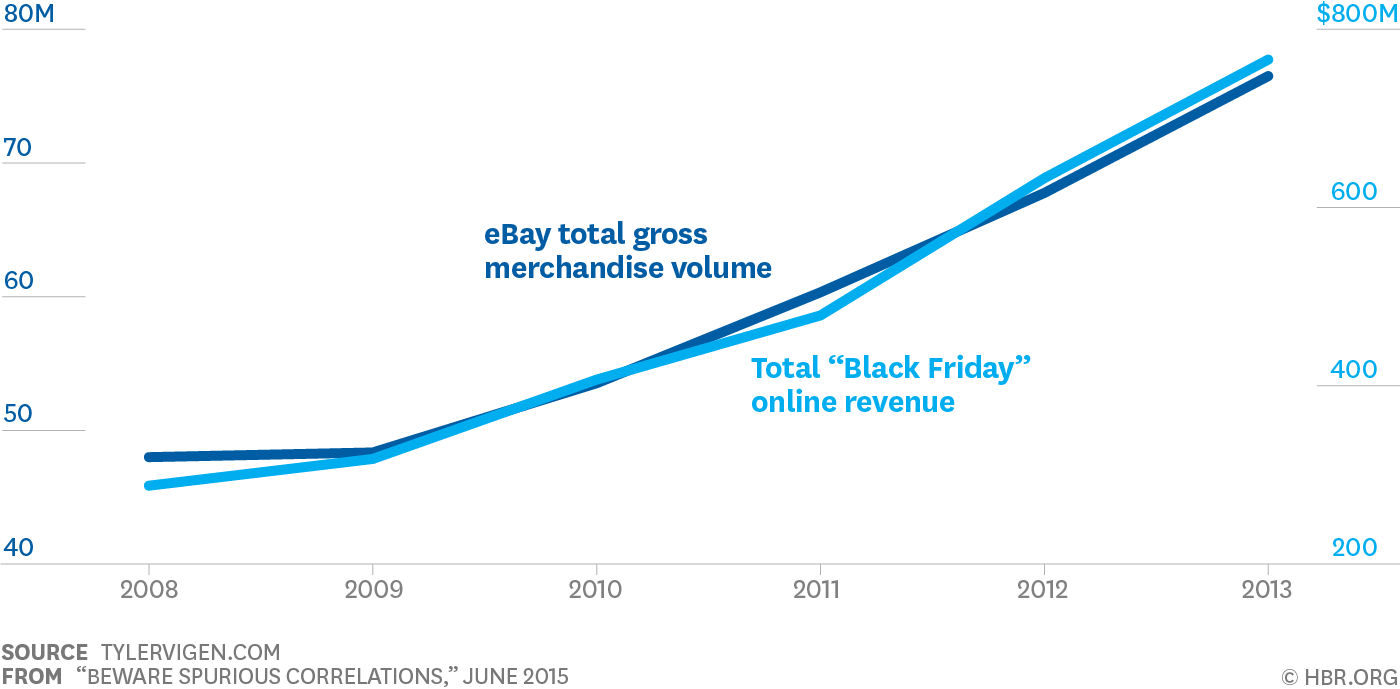
\includegraphics[width=7cm]{P2023.AIBCCSS.InferenceAndLogisticRegression/F1506Z_VS_BEWARESPURIOUSCORRELATIONS-2.png}
\end{center}

\end{frame}

%----------------------------------------------------------------------------------------
%------------------------------------------------
\begin{frame}
{\centerline{Spurious correlations}}
\begin{center}
\LARGE
Correlation does not imply causation.
\end{center}
\end{frame}
%----------------------------------------------------------------------------------------
%------------------------------------------------




%----------------------------------------------------------------------------------------
%------------------------------------------------
\begin{frame}
{\centerline{Spurious correlations}}

\begin{center}
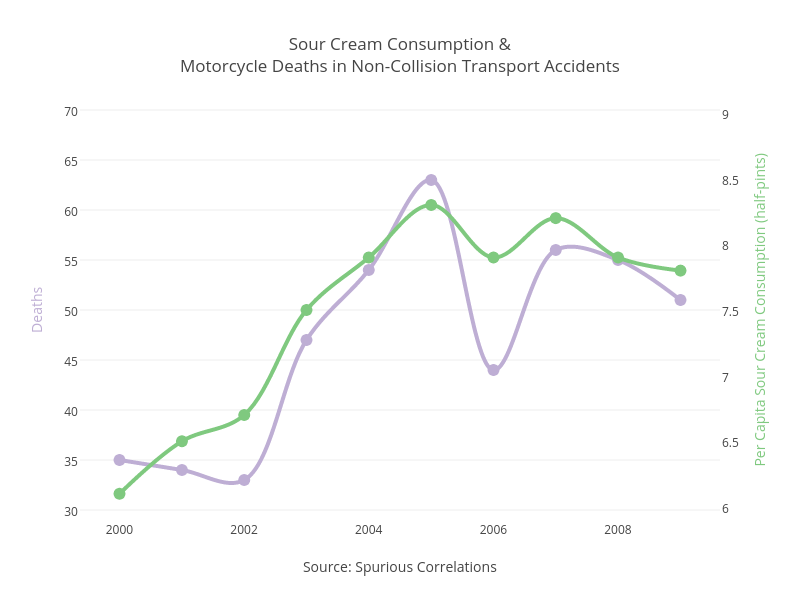
\includegraphics[width=10cm]{P2023.AIBCCSS.InferenceAndLogisticRegression/motor.png}
\end{center}

\end{frame}
%----------------------------------------------------------------------------------------
%------------------------------------------------




%----------------------------------------------------------------------------------------
%------------------------------------------------
\begin{frame}
{\centerline{Spurious correlations}}

\begin{center}
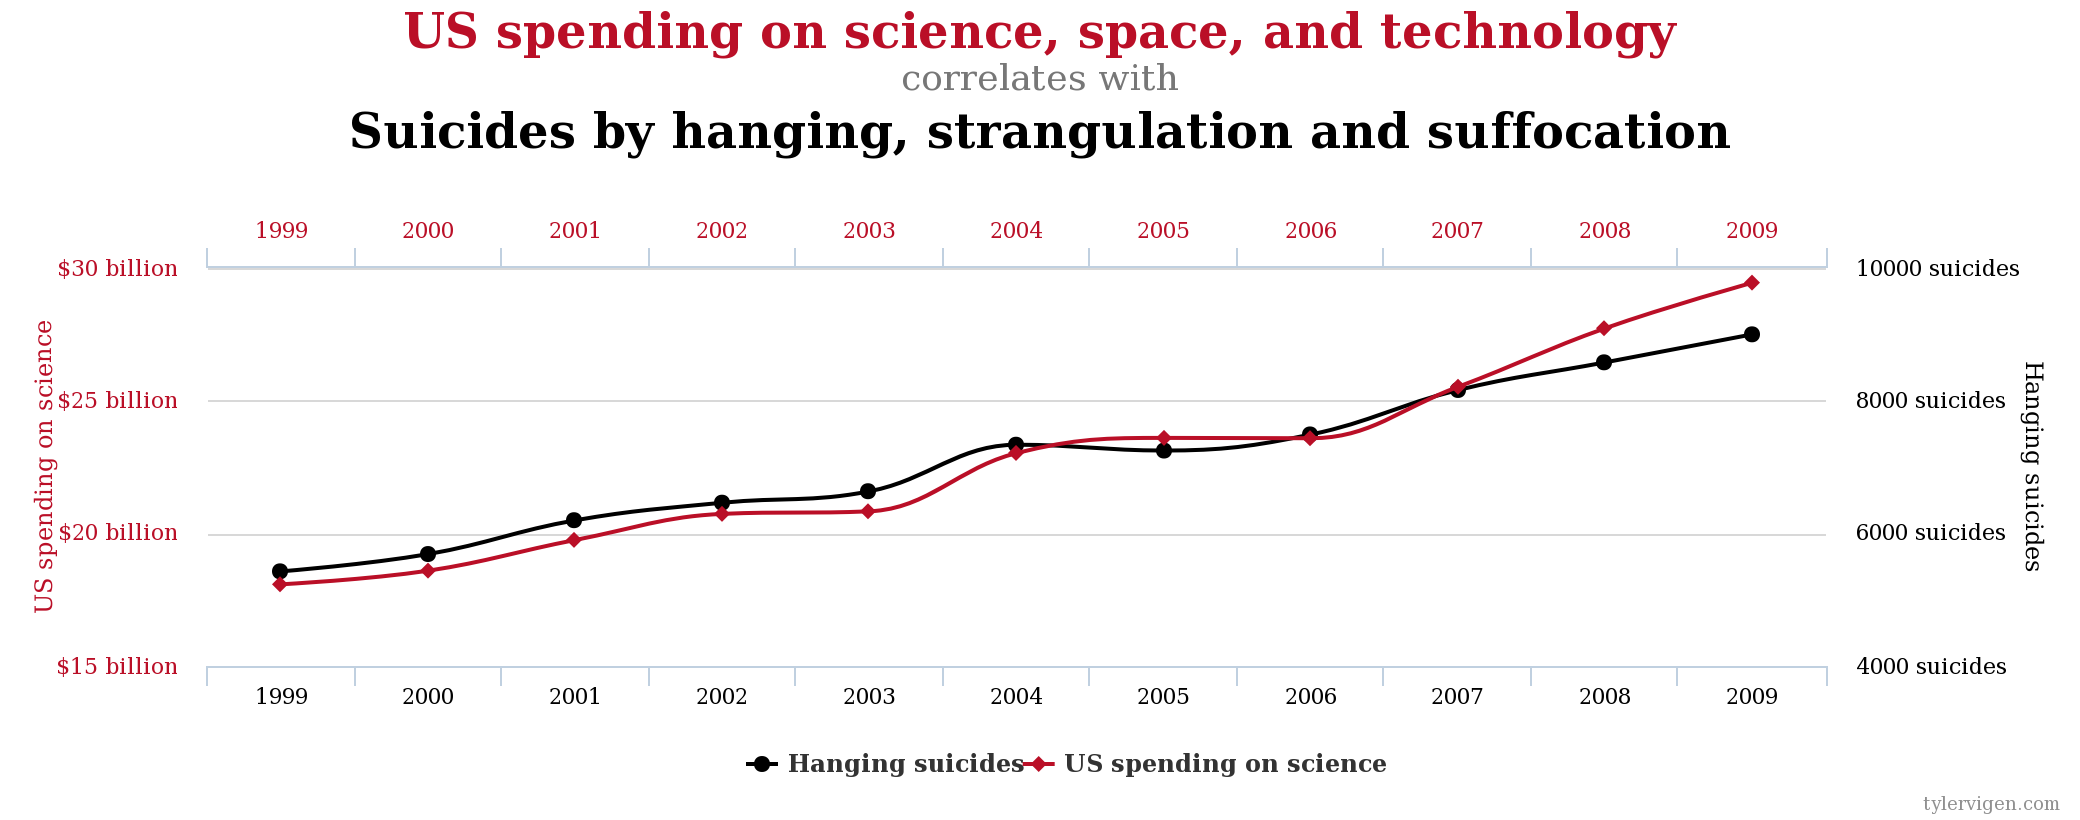
\includegraphics[width=11cm]{P2023.AIBCCSS.InferenceAndLogisticRegression/chart.png}
\end{center}


\end{frame}
%----------------------------------------------------------------------------------------
%------------------------------------------------




%----------------------------------------------------------------------------------------
%------------------------------------------------
\begin{frame}
{\centerline{Spurious correlations}}

\begin{center}
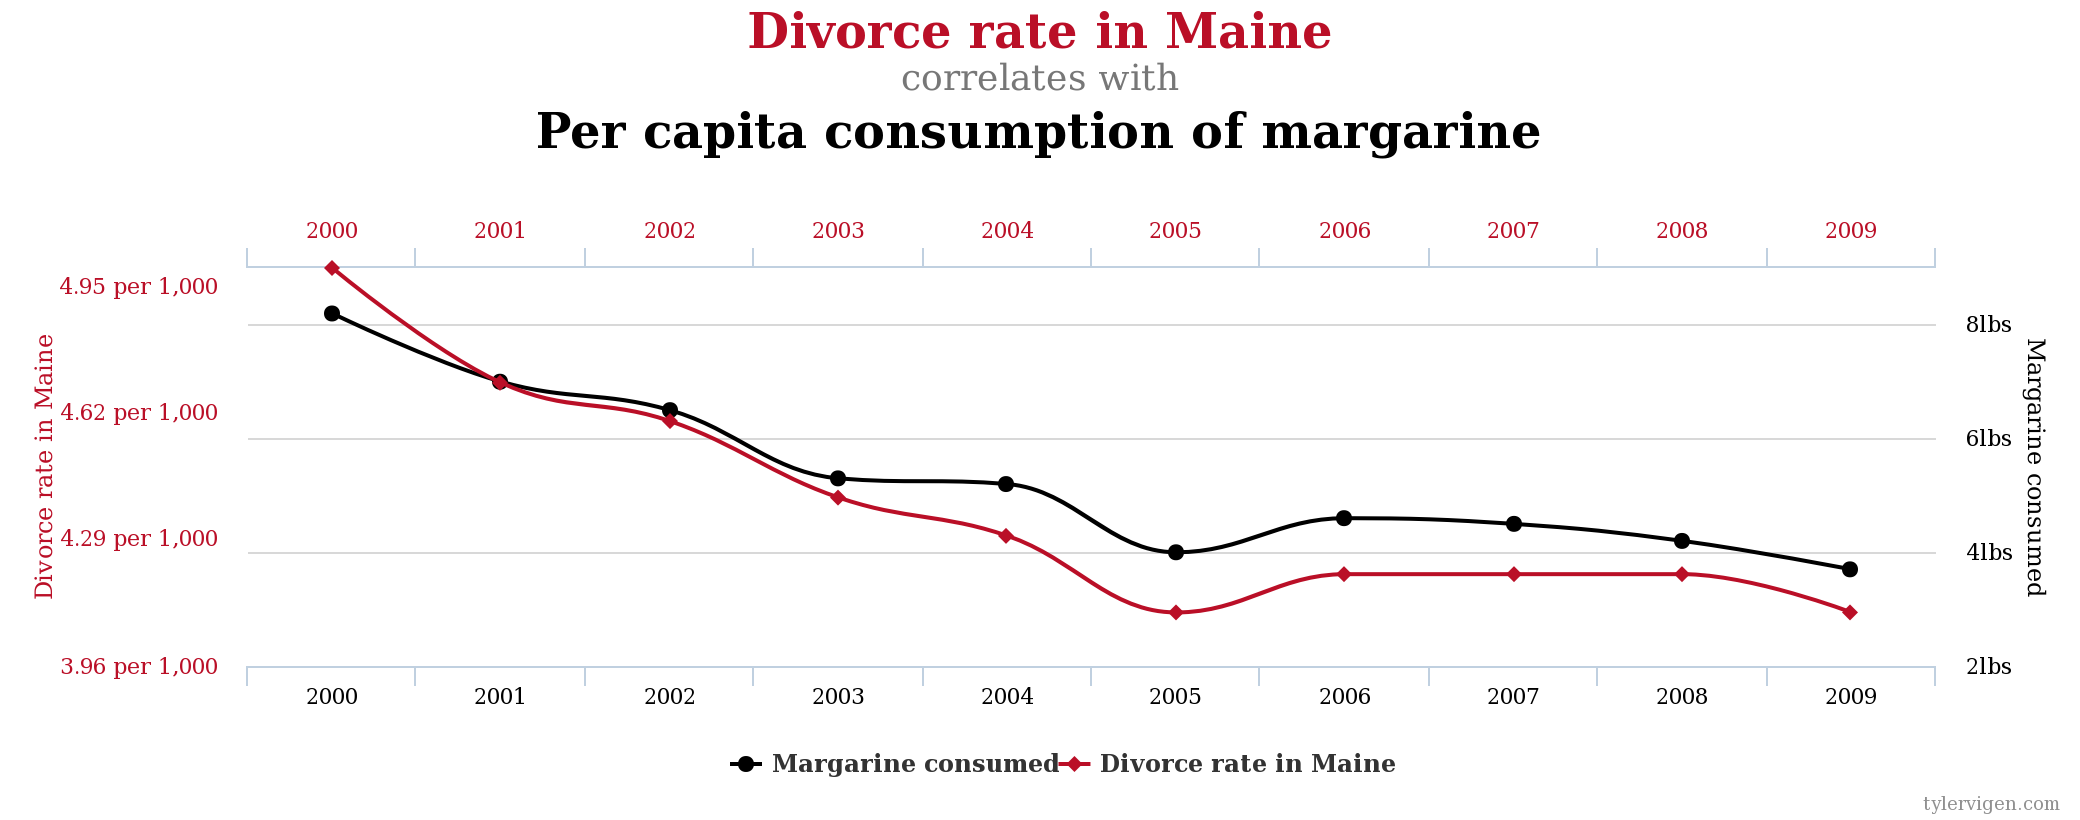
\includegraphics[width=11cm]{P2023.AIBCCSS.InferenceAndLogisticRegression/chart-2.png}
\end{center}


\end{frame}
%----------------------------------------------------------------------------------------
%------------------------------------------------



%----------------------------------------------------------------------------------------
%------------------------------------------------
\begin{frame}
{\centerline{Spurious correlations}}

\begin{center}
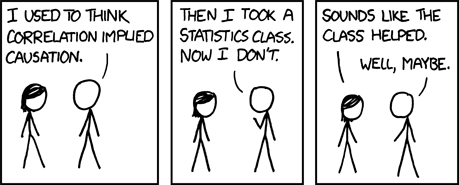
\includegraphics[width=11cm]{P2023.AIBCCSS.InferenceAndLogisticRegression/comics.png}
\end{center}


\end{frame}
%----------------------------------------------------------------------------------------
%------------------------------------------------


\begin{frame}
{\centerline{Distribution of $r_{XY}$ of the sample }}

\begin{itemize}
\item Suppose, as usual, that we have two phenomena that we want to measure,  $X$ and $Y$ and let us assume:
\begin{itemize}
\item that there is a linear relationship between them
\item that I can express the data I collect as:
$$ \hat{Y} = \theta_0 + \theta_1 X + \epsilon $$
where $\epsilon$ is a stationary Gaussian process $N(0,\sigma^2)$
\item that I have $n$ samples, that is $\mathfrak{n}$ set of random pairs $ \mathfrak{S_j} = \{ (\mathfrak{X_{i_j}},\mathfrak{Y_{i_j}}) \}$, with:\\
-- $\mathfrak{j} \in [1 \ldots{} \mathfrak{n} ]$, \\
-- $\mathfrak{i_j} \in [1 \ldots{} \mathfrak{m_j} ]$, \\
-- $(\forall ~ \mathfrak{j}) ~~ \mathfrak{m_j} \in \mathbb{N^+}$
\item for each $ \mathfrak{S_j}$ I can compute the Pearson correlation coefficient $\mathfrak{r_{X_jY_j}}$
\end{itemize}
\item What is the distribution of $\mathfrak{r_{X_jY_j}}$?
\end{itemize}

\end{frame}

\begin{frame}
{\centerline{The Student t (1/3)}}

\begin{itemize}
\item Used to determine the distribution of $\frac{\mathfrak{Dn}}{\mathfrak{s_n}} $ -- We know that $\frac{\mathfrak{Dn}}{\sigma} \xrightarrow{d} N(0,1)$
\item Apparently, started in the brewery of Guinness
\item The pdf is:
$$f_x(x) = \frac { \Gamma \left({\frac {\nu +1}{2}}\right)} {{\sqrt {\nu \pi }} \Gamma \left({\frac {\nu }{2}} \right )} \left ( 1+{\frac {x^{2}}{\nu }} \right )^{-{\frac {\nu +1}{2}}}$$
\item We use the $\Gamma$ function

\end{itemize}
\textit{\tiny
\vspace{-\baselineskip}
Source with modifications: \url{https://en.wikipedia.org/wiki/Student\%27s_t-distribution}}

\end{frame}

\begin{frame}
{\centerline{[The Student t] $\Gamma$  }}

\begin{itemize}
\item  The $\Gamma$ function, an extension of the factorial to the whole $\mathbb{C}$ set apart from negative integers, that it, it is defined on $(\mathbb{R} - \mathbb{N^-},\mathbb{R})$
\item Formally:
$$\Gamma(z) = \int_0^{+ \infty} x ^{z-1} e ^{-x} dx$$

\end{itemize}
\begin{center}
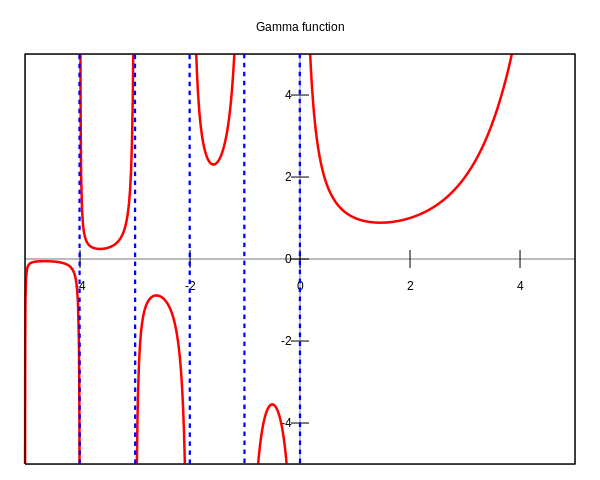
\includegraphics[width=5cm]{P2023.AIBCCSS.InferenceAndLogisticRegression/600px-Gamma_plot.png}
\end{center} 

\textit{\tiny
\vspace{-\baselineskip}
Source with modifications: \url{https://en.wikipedia.org/wiki/Gamma_function}}

\end{frame}

\begin{frame}
{\centerline{The Student t (2/3)}}

\begin{itemize}
\item Recall the pdf:
$$f_x(x) = \frac { \Gamma \left({\frac {\nu +1}{2}}\right)} {{\sqrt {\nu \pi }} \Gamma \left({\frac {\nu }{2}} \right )} \left ( 1+{\frac {x^{2}}{\nu }} \right )^{-{\frac {\nu +1}{2}}}$$
\item The Student t is symmetric
\item $\nu$ is the degree of freedom, as it increases the function becomes similar to the Gaussian (in the figure in Slide \ref{S:GraphT} the t is in red, the Gaussian is in blue, and the previous ts are in green)
\end{itemize}
\textit{\tiny
\vspace{-\baselineskip}
Source with modifications: \url{https://en.wikipedia.org/wiki/Student\%27s_t-distribution}}

\end{frame}

\begin{frame}
{\centerline{The Student t (3/3)}}\label{S:GraphT}

\begin{center}
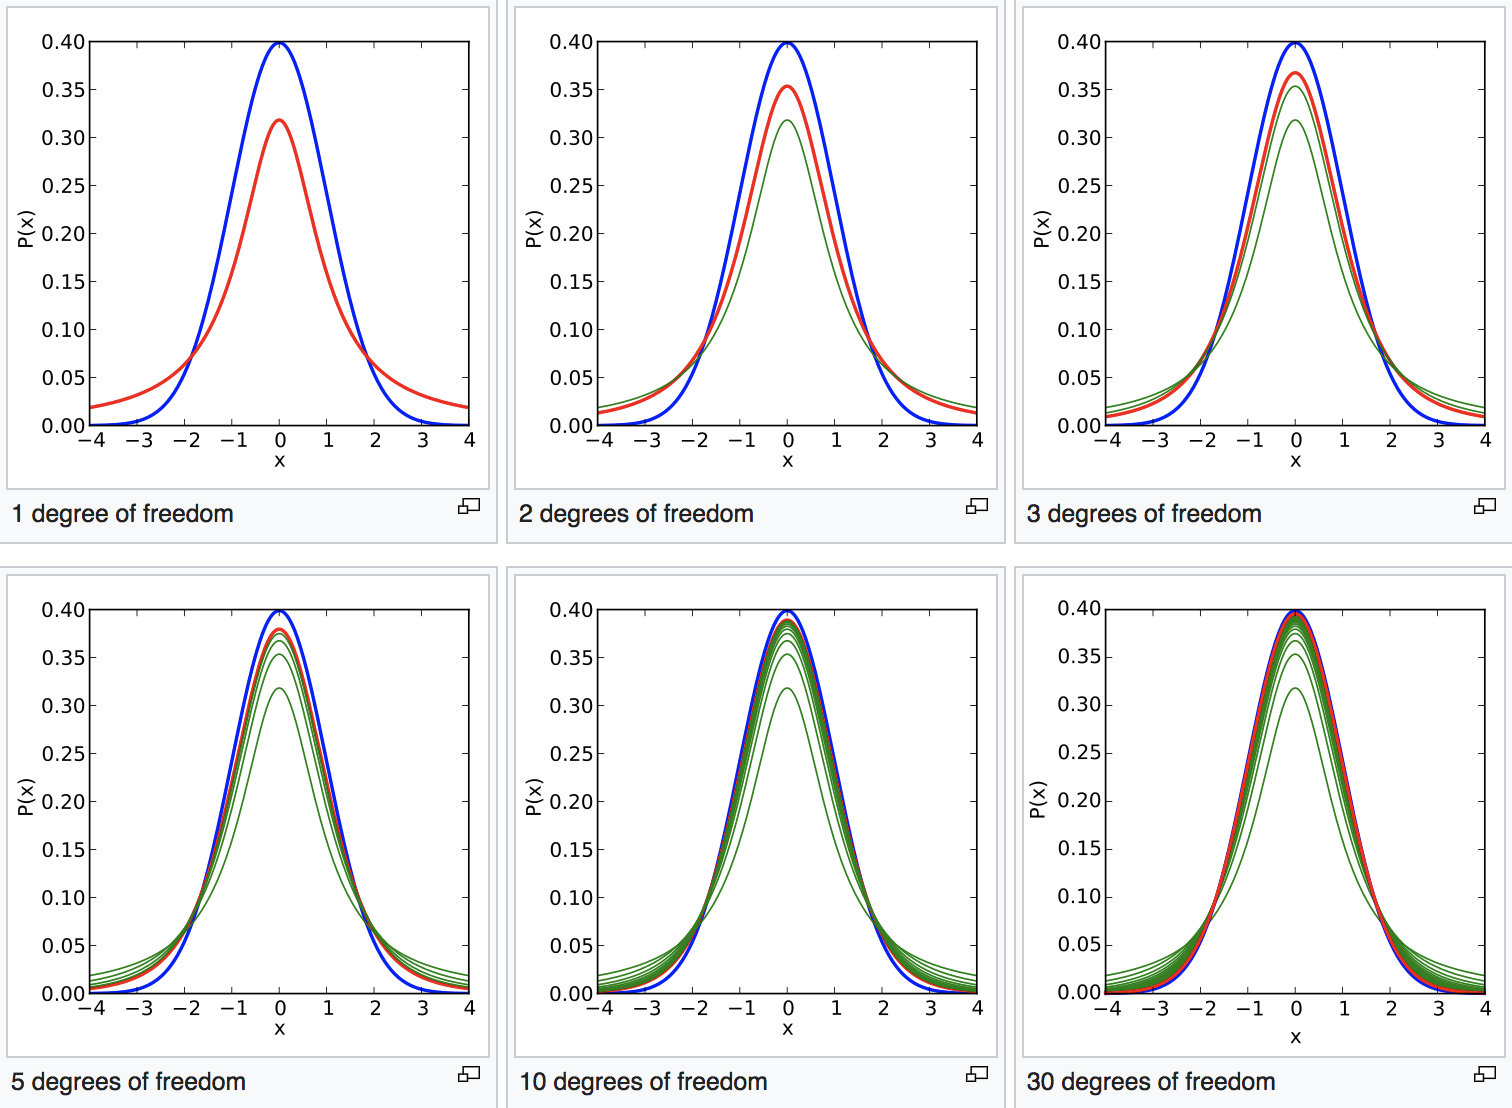
\includegraphics[width=8cm]{P2023.AIBCCSS.InferenceAndLogisticRegression/FromWikipedia_VariousTDistributions.png}
\end{center} 
\textit{\tiny
\vspace{-\baselineskip}
Source with modifications: \url{https://en.wikipedia.org/wiki/Student\%27s_t-distribution}}

\end{frame}


\begin{frame}
{\centerline{Distribution of $\mathfrak{r_{X_jY_j}}$ (1/2) }}

\begin{itemize}
\item The $\mathfrak{r_{X_jY_j}}$ are approximated by a Student t distribution with $(n-2)$ degrees of freedom, under ``good'' assumptions
\item Under such assumptions \textbf{and} the one that we have mentioned before, we have:
$$t = \mathfrak{r_{X_jY_j}}\sqrt{\frac{n-2}{1-\mathfrak{r_{X_jY_j}}^2}}$$
\item and conversely:
$$ \mathfrak{r_{X_jY_j}} = \frac{t}{\sqrt{n - 2 + t^2}}$$
\end{itemize}

\textit{\tiny
\vspace{-\baselineskip}
Source with modifications: \url{https://en.wikipedia.org/wiki/Pearson_correlation_coefficient}}
\end{frame}

\begin{frame}
{\centerline{Distribution of $\mathfrak{r_{X_jY_j}}$ (2/2) }}

\begin{itemize}
\item If we concentrate on:
$$t = \mathfrak{r_{X_jY_j}}\sqrt{\frac{n-2}{1-\mathfrak{r_{X_jY_j}}^2}}$$
\item we notice that for the same value of $\mathfrak{r_{X_jY_j}}$ we obtain higher values of $t$, with increasing values of $n$
\end{itemize}
\begin{center}
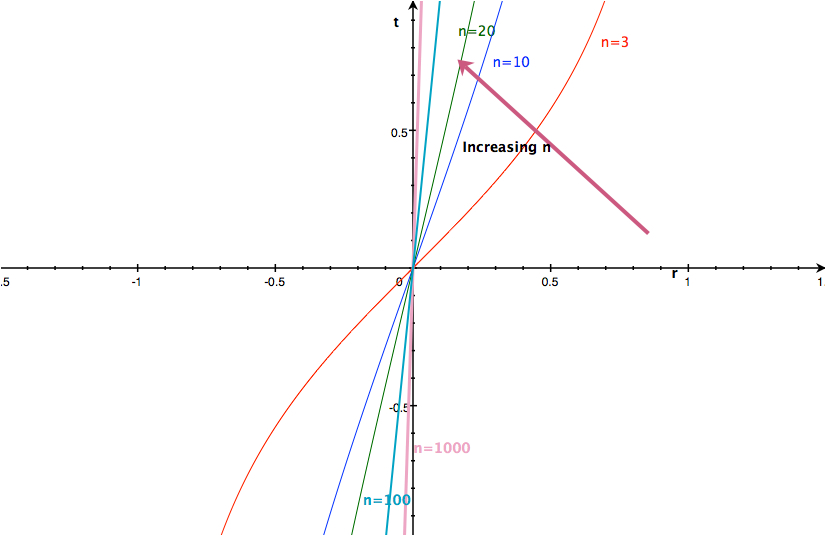
\includegraphics[width=6cm]{P2023.AIBCCSS.InferenceAndLogisticRegression/StudentTCorrelation.jpg}
\end{center} 

\end{frame}

\begin{frame}
{\centerline{Distribution of $\mathfrak{r_{X_jY_j}}$ }}

\underline{Claim:} \\
$$t_{n-2} \sim \frac{r\sqrt{n-2}}{\sqrt{1-r^2}}$$

\underline{Assamptions and Facts:} \\
\vspace*{2mm}
\begin{itemize}
\item $ Y = \beta_0 + \beta_1 X + \epsilon $. 
%\newline

\item $\hat{Y} = \hat{\beta_0} + \hat{\beta_1} X$

\item Where $\beta_0 \in \mathbb{R}$ , $\beta_1 \in \mathbb{R} \setminus \{0\}$ and $\epsilon \sim N(0, \sigma^2)$. 
\end{itemize}

\vspace*{2.5mm}

\end{frame}


\begin{frame}
{\centerline{$ \frac{r\sqrt{n-2}}{\sqrt{1-r^2}} \sim t_{n-2}  $  ~~ --- ~~ Proof (1/7)}}

\underline{\textcolor{red}{Plan:}}
\begin{itemize}
\setlength\itemsep{0.8em}
\item $\hat{\beta_1} \sim \mathcal{N}$
\item $RSS \sim \chi^2$
\item $t \sim \frac{\hat{\beta_1}}{RSS}$
\end{itemize}



\end{frame}

\begin{frame}
{\centerline{$ \frac{r\sqrt{n-2}}{\sqrt{1-r^2}} \sim t_{n-2} $  ~~ --- ~~ Proof (2/7)}}

Given model $y = \beta_0 + \beta_1 x_i + \epsilon$, $\beta_1$ estimator ($\hat{\beta_1}$) can be derived as follows :
$$\hat{\beta_1} = \frac{s_{xy}}{s_{xx}}$$

\textcolor{red}{Remember : }
\begin{itemize}
\setlength\itemsep{0.8em}
\item $s_{xx} = \sum \left ( x_i - \bar{x} \right )^{2} $
\item $s_{xy} = \sum \left ( x_i - \bar{x} \right ) \left ( y_i - \bar{y} \right ) $
\end{itemize}

$$\hat{\beta_1} = \frac{s_{xy}}{s_{xx}} = \sum \frac{(x_i - \bar{x})}{s_{xx}} \left ( y_i - \bar{y} \right ) = \sum \frac{(x_i - \bar{x})}{s_{xx}} y_i  - \sum \frac{(x_i - \bar{x})}{s_{xx}} \bar{y}$$

\begin{center}
\tiny{Taken with modifications from \url{https://math.stackexchange.com/questions/787939/show-that-the-least-squares-estimator-of-the-slope-is-an-unbiased-estimator-of-t/788010\#788010}}
\end{center}
\end{frame}

\begin{frame}
{\centerline{$  \frac{r\sqrt{n-2}}{\sqrt{1-r^2}} \sim t_{n-2}  $  ~~ --- ~~ Proof (3/7)}}

Therefore :
\begin{align*}\
\hat{\beta_1} & = \frac{s_{xy}}{s_{xx}} = \sum \frac{(x_i - \bar{x})}{s_{xx}} \left ( y_i - \bar{y} \right ) = \sum \frac{(x_i - \bar{x})}{s_{xx}} y_i  - 0 * \bar{y} \\
& = \sum \frac{(x_i - \bar{x})}{s_{xx}} y_i  = \sum \frac{(x_i - \bar{x})}{s_{xx}} \left ( \textcolor{cyan}{\beta_0} + \textcolor{red}{\beta_1 x_i} + \textcolor{blue}{\epsilon_i }\right ) \\
& = \textcolor{cyan}{\beta_0 \sum \frac{(x_i - \bar{x})}{s_{xx}}}  + \textcolor{red}{ \beta_1 \sum \frac{(x_i - \bar{x})}{s_{xx}}x_i} + \textcolor{blue}{\sum \frac{(x_i - \bar{x})}{s_{xx}}\epsilon_i }
\end{align*}

Note 1:
$$ \textcolor{cyan}{\sum \frac{(x_i - \bar{x})}{s_{xx}}} = \frac{1}{s_{xx}} \sum \left ( x_i - \bar{x} \right ) =  \frac{1}{s_{xx}} \left ( \sum x_i - \sum \bar{x} \right ) = \textcolor{cyan}{0}$$


% \begin{align*}\
% \hat{\beta_1} &= \frac{s_{xy}}{s_{xx}} = \sum \frac{(x_i - \bar{x})}{s_{xx}} \left ( Y_i - \bar{y} \right ) \\
% & = \sum \frac{(x_i - \bar{x})}{s_{xx}} y_i  - \sum \frac{(x_i - \bar{x})}{s_{xx}} \bar{y}
% \end{align*}

\begin{center}
\tiny{Taken with modifications from \url{https://math.stackexchange.com/questions/787939/show-that-the-least-squares-estimator-of-the-slope-is-an-unbiased-estimator-of-t/788010\#788010}}
\end{center}
\end{frame}


\begin{frame}
{\centerline{$  \frac{r\sqrt{n-2}}{\sqrt{1-r^2}} \sim t_{n-2} $  ~~ --- ~~ Proof (4/7)}}

Note 2:
\begin{align*}\
\textcolor{red}{\sum \frac{(x_i - \bar{x})}{s_{xx}}x_i} &= \sum \frac{(x_i - \bar{x})}{s_{xx}} \left ( x_i - \bar{x} + \bar{x} \right ) \\
&= \sum \frac{(x_i - \bar{x})}{s_{xx}} \left ( x_i - \bar{x} \right ) + \sum \frac{(x_i - \bar{x})}{s_{xx}} \bar{x} \\
&=  \frac{1}{s_{xx}} \sum \left ( x_i - \bar{x} \right )^2 = \textcolor{red}{1}
\end{align*}

Putting the simplifications into the original equation:
$$\hat{\beta_1} =  \textcolor{cyan}{0 \times \beta_0} + \textcolor{red}{1 \times \beta_1} + \textcolor{blue}{\sum \frac{(x_i - \bar{x})}{s_{xx}}\epsilon_i} = \textcolor{red}{\beta_1} + \textcolor{blue}{\sum \frac{(x_i - \bar{x})}{s_{xx}}\epsilon_i} $$

\end{frame}



\begin{frame}
{\centerline{$  \frac{r\sqrt{n-2}}{\sqrt{1-r^2}} \sim t_{n-2} $  ~~ --- ~~ Proof (5/7)}}

\begin{itemize}
\item Remember that:
\begin{itemize}
\item $ \textcolor{olive}{ \sum_i \frac{ \left ( x_i - \bar{x} \right)^2}{s_{xx}} = 1}$
\item $\hat{\beta_1} = \textcolor{red}{\beta_1} + \textcolor{blue}{\sum_i \frac{(x_i - \bar{x})}{s_{xx}} \epsilon_i}$
\item $ \forall \textcolor{blue}{i}, ~~ \textcolor{blue}{\epsilon_i} \sim \mathcal{N}(0, \sigma^2)$
\item $ \forall \textcolor{cyan}{\lambda}  \neq 0, ~~ \textcolor{cyan}{\lambda} \mathcal{N}\left ( \mu,\sigma^{2} \right )  = \mathcal{N}\left ( \textcolor{cyan}{\lambda}  \mu,\left (\textcolor{cyan}{\lambda}  \sigma\right )^{2} \right )$
\item $\sum_i \mathcal{N}\left ( \mu_i,\sigma^{2}_i \right ) = \mathcal{N}\left ( \sum_i \mu_i , \sum_i \sigma^{2}_i \right )$
\end{itemize}
\end{itemize}
\end{frame}

\begin{frame}
{\centerline{$  \frac{r\sqrt{n-2}}{\sqrt{1-r^2}} \sim t_{n-2} $  ~~ --- ~~ Proof (6/7)}}

\begin{itemize}
\item Therefore:
\begin{itemize}
\item  $\textcolor{blue}{\sum \frac{(x_i - \bar{x})}{s_{xx}} \epsilon_i} \sim  \mathcal{N} \left (0,  \sum_i \left ( \frac{\sigma (x_i - \bar{x})}{s_{xx}} \right )^2 \right ) = $
$ =  \mathcal{N} \left (0,  \sigma^2 \sum_i \left ( \frac{ x_i - \bar{x} }{s_{xx}} \right )^2 \right )  = \mathcal{N} \left (0, \frac{\sigma^2}{s_{xx}} \textcolor{olive}{\sum_i \frac{\left ( x_i - \bar{x} \right)^2}{s_{xx}}} \right ) = \mathcal{N} \left ( 0, \frac{\sigma^2}{s_{xx}} \right )$

\item $\hat{\beta_1} \sim \mathcal{N}  \left ( \beta_1, \frac{\sigma^2}{s_{xx}} \right )$
\item $\frac{\hat{\beta_1} - \beta_1}{\sigma / \sqrt{s_{xx}}} \sim \mathcal{N} \left ( 0, 1 \right ) $
\end{itemize}
\end{itemize}




\end{frame}


\begin{frame}
{\centerline{$  \frac{r\sqrt{n-2}}{\sqrt{1-r^2}} \sim t_{n-2}  $  ~~ --- ~~ Status (1/3)}}

\begin{itemize}
    \item Note the following:
\begin{itemize}
    \item  We know that $t_n$ can be rewritten using a \textcolor{red}{$\chi^2_n$} distribution:
               $$t_n  ~\sim~  \frac{\mathcal{N}\left ( 0,1 \right )}{\sqrt{\textcolor{red}{\chi^2_n /n}}} $$
    \item And also we can connect \textit{RSS}, $\sigma$, and $\chi^2$:
    $$\frac{RSS}{\sigma^2} = \frac{\sum \epsilon^2_i}{\sigma^2} = \sum \left ( \frac{ \epsilon_i}{\sigma} \right )^2 = \sum \left ( \mathcal{N}(0, 1) \right )^2 ~\sim~ \textcolor{red}{\chi^2_{n-2}}$$

\end{itemize}
\end{itemize}



% Under null hypothesis $H_0 : \beta_1 = 0$
\vspace*{0.5cm}
\begin{center}
\tiny{Taken with modifications from \url{https://stats.stackexchange.com/questions/204238/why-divide-rss-by-n-2-to-get-rse}}
\end{center}
\end{frame}

\begin{frame}
{\centerline{$  \frac{r\sqrt{n-2}}{\sqrt{1-r^2}} \sim t_{n-2}  $  ~~ --- ~~ Status (2/3)}}

\begin{itemize}
\item We will now proceed as follows:
\begin{itemize}
\setlength\itemsep{0.5em}
\item $\hat{\beta_1} \sim \mathcal{N}$
\item $RSS \sim \chi^2$
\item $t \sim \frac{\hat{\beta_1}}{RSS}$
\end{itemize}
\end{itemize}



% Under null hypothesis $H_0 : \beta_1 = 0$
\vspace*{0.5cm}
\begin{center}
\tiny{Taken with modifications from \url{https://stats.stackexchange.com/questions/204238/why-divide-rss-by-n-2-to-get-rse}}
\end{center}
\end{frame}



\begin{frame}
{\centerline{$  \frac{r\sqrt{n-2}}{\sqrt{1-r^2}} \sim t_{n-2}  $  ~~ --- ~~ Status (3/3)}}

\begin{itemize}
\setlength\itemsep{0.8em}
\item $r^2 = 1 - \frac{RSS}{SST}$
\item $RSS = (1 - r^2)s_{yy} $
\item $SST = s_{yy} = \sum ( y_i - \bar{y} )^2 \frac{RSS}{SST}$
\item $r = \frac{s_{xy}}{\sqrt{s_{xx}s_{yy}}} = \frac{\sum (x_i - \bar{x})(y_i - \bar{y})}{\sqrt{\sum (x_i - \bar{x})^2 + \sum (y_i - \bar{y})^2}}$
% \item $\frac{RSS}{\sigma^2} = \chi^2_{n-2}$
% \item $t_n = \frac{\mathcal{N}(0, 1)}{\sqrt{\chi^2_{n}/n}}$
\item $t_{n-2} \sim \frac{\frac{\hat{\beta_1} - \beta_1}{\sigma / \sqrt{s_{xx}}}}{\sqrt{RSS / (n-2)\sigma^2}} = \frac{r\sqrt{(n-1)}}{\sqrt{(1 - r^2)}}$
\end{itemize}

% Under null hypothesis $H_0 : \beta_1 = 0$

\begin{center}
\tiny{Taken with modifications from \url{https://stats.stackexchange.com/questions/204238/why-divide-rss-by-n-2-to-ge t-rse}}
\end{center}
\end{frame}


\begin{frame}
{\centerline{$  \frac{r\sqrt{n-2}}{\sqrt{1-r^2}} \sim t_{n-2}  $  ~~ --- ~~ Proof (7/7)}}

Under null hypothesis $H_0 : \beta_1 = 0$
\begin{align*}\
\frac{\frac{\hat{\beta_1} - 0}{\sigma / \sqrt{s_{xx}}}}{\sqrt{\frac{RSS}{\sigma^2 (n - 2)}}} &= \frac{\hat{\beta_1} \sqrt{s_{xx}}}{\sigma} . \frac{\sqrt{\sigma^2 (n-2)}}{\sqrt{RSS}} = \frac{\hat{\beta_1} \sqrt{s_{xx}}}{1} . \frac{\sqrt{(n-2)}}{\sqrt{(1 - r^2)s_{yy}}} \\
& = \frac{\hat{\beta_1} \sqrt{s_{xx}}}{\sqrt{s_{yy}} } . \frac{\sqrt{(n-2)}}{\sqrt{(1 - r^2)}} = \frac{\frac{s_{xy}}{s_{xx}}\sqrt{s_{xx}}}{\sqrt{s_{yy}} } . \frac{\sqrt{(n-2)}}{\sqrt{(1 - r^2)}} \\
& =  \frac{s_{xy}}{\sqrt{s_{yy}s_{xx}} } . \frac{\sqrt{(n-2)}}{\sqrt{(1 - r^2)}} = \frac{r\sqrt{(n-2)}}{\sqrt{(1 - r^2)}} \\
& \textbf{\textcolor{red}{QED}}
\end{align*}


\end{frame}



\begin{frame}
{\centerline{Reasoning on $\theta_1$ (1/2)}}

$$ \theta_1  = \frac{Cov(X,Y)}{Var(X)} = \frac{\sigma_Y}{\sigma_X} r_{X,Y}$$
\begin{center}
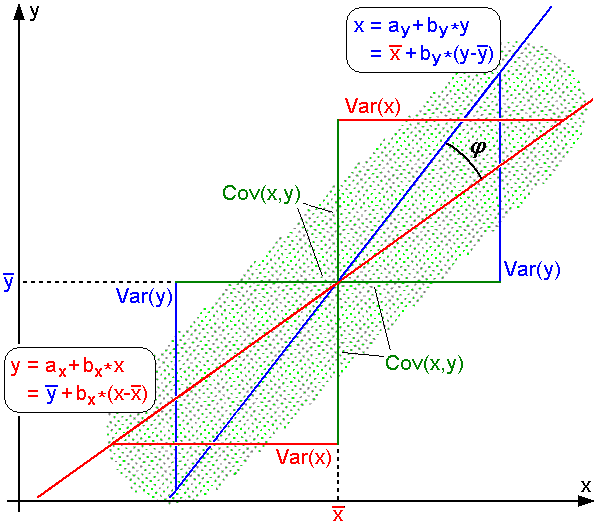
\includegraphics[width=5.5cm]{P2023.AIBCCSS.InferenceAndLogisticRegression/Regression_lines.png}
\end{center} 

\textit{\tiny
\vspace{-\baselineskip}
Source with modifications: \url{https://en.wikipedia.org/wiki/Pearson_correlation_coefficient}}

\end{frame}

\begin{frame}
{\centerline{Reasoning on $\theta_1$ (2/2)}}

\begin{itemize}
\item Remember that:
$$ \theta_1  = \frac{\sigma_Y}{\sigma_X} r_{X,Y}   $$
\item If $r_{X,Y} > 0$, we define the $p$-value of our correlation the $P( \theta_1 < 0)$, conversely, if $r_{X,Y} < 0$ we define the $p$-value of our correlation the $P( \theta_1 > 0)$
\item In other terms, the $p$-value of a correlation is the probability that a slope change direction
\end{itemize}

\textit{\tiny
\vspace{-\baselineskip}
Source with modifications: \url{https://en.wikipedia.org/wiki/Pearson_correlation_coefficient}}

\end{frame}


\begin{frame}
{\centerline{The power function of a test}}
Remember that:
\begin{itemize}
\item A type 1 error is when we reject the null hypothesis when the null hypothesis is true, that is we think that something is going on, but nothing is really there. The probability of committing a type 1 error is typically referred to as $\alpha$.
\item A type 2 error is when we fail to reject the null hypothesis when actually we should reject it, that is, we fail to perceive a phenomena. The probability of committing a type 2 error is typically referred to as $\beta$.
\end{itemize}

The power function of a test informally is the probability of not committing a type 2 error, that is, $(1-\beta)$

\end{frame}


\begin{frame}
{\centerline{Power of a test}}

\begin{itemize}
    \item In general the non rejection of the null hypothesis H0 does not mean that H0 holds
    \item The power of a binary test is the probability that the tests rejects the null hypothesis when the alternate hypothesis is true\\
    \begin{center}
    \textcolor{red}{Power(Test) = P(reject H0 \textbar~ H1 is true)}
    \end{center}
    \item If a test has power of 0.99 in a given situation, it means that the non rejections of H0 means that H0 holds with a p(error) $\leq$ 0.01
    \item The power of a test has an essential role in determining the test to select and in interpreting its results
\end{itemize}

\begin{center}
\tiny{Taken with modifications from \url{https://en.wikipedia.org/wiki/Power_(statistics)}}
\end{center}

\end{frame}
%=============================================

\begin{frame}
{\centerline{What influences the power of a test}}

The power of a test is influenced by a variety of factors, such as:
\begin{itemize}
    \item the size of the datasets
    \item the magnitude of the effect
    \item the level of statistical significance
    \item the intrinsic structure of a test
    \begin{itemize}
        \item we can use a test only if its hypotheses are all verified
        \item informally, the more stringent the hypotheses, the higher the power of the test, since $\ldots$
        \item $\ldots$ \textit{we know better the population}
    \end{itemize}

\end{itemize}

\begin{center}
\tiny{Taken with modifications from \url{https://en.wikipedia.org/wiki/Power_(statistics)}}
\end{center}

\end{frame}
%=============================================

%=============================================

\begin{frame}
{\centerline{Parametric and non parametric tests}}

We can distinguish two major classes of tests:
\begin{itemize}
    \item When we \textcolor{red}{\bf can make assumptions} on the distributions of the two datasets;
    \begin{itemize}
    \item for this case, we have the \textit{parametric} tests, since we can assume parameters of the underlying distribution
    \end{itemize}
    \item When we \textcolor{red}{\bf cannot}
    \begin{itemize}
    \item for this case, we have the \textit{non parametric} tests, since we cannot make any assumption on any kind of parameter of the underlying distribution
\end{itemize}

\end{itemize}

\begin{center}
\tiny{Taken with modifications from \url{https://en.wikipedia.org/wiki/Power_(statistics)}}
\end{center}

\end{frame}

\begin{frame}
{\centerline{The problem of multiple testing }}
Consider a case where you have \textbf{20} hypotheses to test, and a significance level of \textbf{0.05}. 
\newline

The probability of observing at least one significant result just due to chance?

$$\mathbb{P}(at\_least\_1\_signif.\_results) = 1 - \mathbb{P}(no\_signif.\_results) = $$
$$= 1 - (1-0.05)^{20} \approx 0.64$$


\end{frame}
%----------------------------------------------------------------------------------------

%----------------------------------------------------------------------------------------
\begin{frame}
{\centerline{The Bonferroni correction }}
So, with 20 tests being considered, we have a \textbf{64\%} chance of observing at least one significant result, even if all of the tests are actually not significant.
\newline

The Bonferroni correction sets the significance cut-off at $\alpha/n$. 
\newline

For example, with \textbf{20} tests and $\alpha = 0.05$, you’d only reject a null hypothesis if the p-value is less than \textbf{0.0025}.


\end{frame}


%----------------------------------------------------------------------------------------
\begin{frame}
{\centerline{Toward the Bonferroni inequality (1/2)}}
\underline{Claim (Boole Inequality):} 
Let $A_1$, $A_2$, $\ldots$, $A_n$ be $n$ events, then:
$$ P({\bigcup_{i \mathop = 1}^n A_i}) \le \sum_{i \mathop = 1}^n P({A_i}) $$
\underline{Proof:}
\textit{By induction}\\
\textit{Base}\\
For n=1 it is trivially verified. \\
For n=2:
$$ P(A_1 \cup A_2) =   P(A_1) + P (A_2) - P(A_1 \cap A_2) \le P(A_1) + P (A_2)$$
since $P(A_1 \cap A_2) \ge 0$.


\end{frame}

% %----------------------------------------------------------------------------------------

\begin{frame}
{\centerline{Toward the Bonferroni inequality (2/2) }}
\textit{Step}\\
Assuming it true for $n \ge 2$, we prove it for $n+1$.\\
Given the associativity of the $\cup$:
$$ P({\bigcup_{i \mathop = 1}^{n+1} A_i}) = P({\bigcup_{i \mathop = 1}^{n} A_i \cup A_{n+1}})$$
Calling $B$ the set $\bigcup_{i \mathop = 1}^{n} A_i$ and $C$ the set $ A_{n+1}$ we can write:
$$P(B \cup C) =   P(B) + P (C) - P(B \cap C) \le P(B) + P (C)$$
Which means:
$$ P({\bigcup_{i \mathop = 1}^{n+1} A_i}) \le P({\bigcup_{i \mathop = 1}^{n} A_i}) + P(A_{n+1}) \le \sum_{i \mathop = 1}^n P({A_i}) + P(A_{n+1}) = \sum_{i \mathop = 1}^{n+1} P({A_i})$$
\underline{QED}
\end{frame}

% %----------------------------------------------------------------------------------------

%----------------------------------------------------------------------------------------
\begin{frame}
{\centerline{The Bonferroni correction - Proof}}
\underline{Claim (Bonferroni correction):} In the case of $m$ null hypotheses $H0_1 \cdots H0_m$ sufficient condition to have a probability than a given $\alpha$ of wrongly rejecting a null hypothesis is that $\forall i \in [1 \cdots m], p_i \leq \frac{\alpha}{m}$.
\newline 
\underline{Proof:}

From the Boole inequality:
$$P \big(\bigcup_{i=1}^{m}(p_i\leq\frac \alpha m ) \big) \leq\sum_{i=1}^{m}\left\{P\left(p_i\leq\frac \alpha m\right)\right\} \leq m \frac \alpha m = \alpha$$

\underline{QED}
\end{frame}

\begin{frame}
{\centerline{References}}

1) \url{http://www.cs.umd.edu/~djacobs/CMSC426/Convolution.pdf}
\newline 

2) \url{https://www.researchgate.net/post/Difference\_between\_convolution\_and\_correlation}
\newline 

3) \url{https://www.tutorialspoint.com/signals\_and\_systems/convolution\_and\_correlation.htm}

\end{frame}

\begin{frame}
{\centerline{Part 2}}

\begin{center}
\Huge Non parametric correlations
\end{center}
\end{frame}

\begin{frame}
{\centerline{Spearman's Rank Correlation Coeff. (1/3)}}

\begin{itemize}
   \item What can we do when the data is not normally distributed?
   \item Or even if the data is not on a ratio scale, just on an ordinal scale?\newline
   \item \textit{If the data is on a nominal scale, the concept of correlation looses interest; at most we can consider clustering.}
\end{itemize}


\end{frame}

\begin{frame}
{\centerline{Spearman's Rank Correlation Coeff. (2/3)}}
Idea:
\begin{itemize}
   \item Transform the data into ranks
   \item Apply the Pearson correlation coefficient to ranks
   \item Indeed, the values can be different, and also the significance and the mutual relationship
   \item Remember that:
   $$r_{X,Y} = \frac{Cov(X,Y)}{\sigma_X\sigma_Y}$$
   \item And also that:
   $$ \theta_1  = \frac{\sigma_X\sigma_Y}{Var(X)} r_{X,Y}   $$
\end{itemize}

\textit{\tiny
\vspace{-\baselineskip}
Source with modifications: \url{https://en.wikipedia.org/wiki/Spearman\%27s_rank_correlation_coefficient}}

\end{frame}

\begin{frame}
{\centerline{Spearman's Rank Correlation Coeff. (3/3)}}
Definition:
\begin{itemize}
   \item Let's have two sets $X = \{X_i\}$ and $Y= \{Y_i\}$ of the same size $n$ where $(\forall i) X_i,Y_i \in \text{ordinal scale}$
   \item Let's consider a set of pairs $P_{X,Y} = \{(X_i,Y_i)\}$ 
   \item Let's define 
   \begin{itemize}
   \item $(\forall X_i \in X) ~ rk{_X{_i}} = \text{rank}(X_i,X)$, $Rk_X = \{ rk_{X{_i}} \} $ 
   \item $(\forall Y_i \in Y) ~ rk_{Y{_i}} = \text{rank}(Y_i,Y)$, $Rk_Y = \{ rk_{Y{_i}} \} $ 
\end{itemize}
    \item We define the Spearman's Rank Correlation Coefficient between $X$ and $Y$, $r_S(X,Y)$ as:
    $$r_S(X,Y) = r(Rk_X, Rk_Y) = \frac{Cov(Rk_X,Rk_Y)}{\sigma_{Rk_X}\sigma_{Rk_Y}}$$
\end{itemize}

\textit{\tiny
\vspace{-\baselineskip}
Source with modifications: \url{https://en.wikipedia.org/wiki/Spearman\%27s_rank_correlation_coefficient}}

\end{frame}

\begin{frame}
{\centerline{Visualization of $r_S$}}

Spearman's Rank Correlation Coefficient is based on monotonicity:

\begin{center}
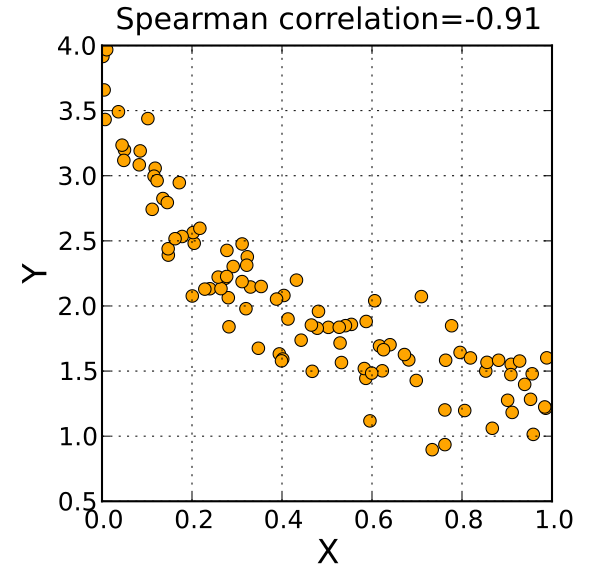
\includegraphics[width=0.45\textwidth]{P2023.AIBCCSS.InferenceAndLogisticRegression/600px-Spearman_fig4.png}
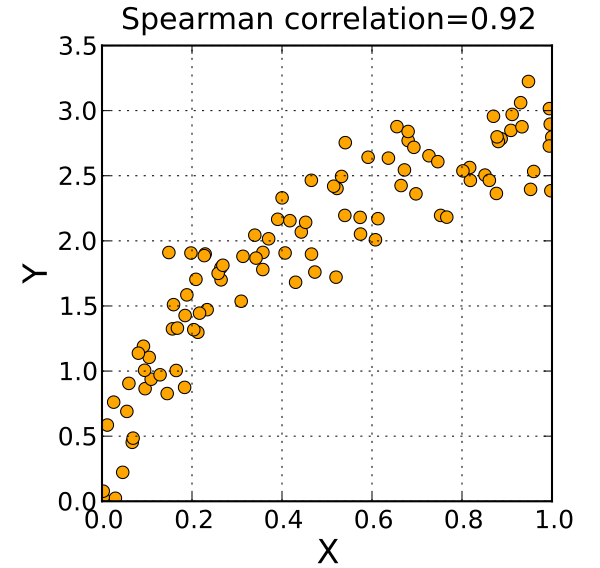
\includegraphics[width=0.45\textwidth]{P2023.AIBCCSS.InferenceAndLogisticRegression/600px-Spearman_fig5.png}
\end{center} 

\textit{\tiny
\vspace{-\baselineskip}
Source with modifications: \url{https://en.wikipedia.org/wiki/Spearman\%27s_rank_correlation_coefficient}}

\end{frame}


\begin{frame}
{\centerline{$r$ and $r_S$ (1/2)}}

Indeed, the values of $r$ and $r_S$ can be different:

\begin{center}
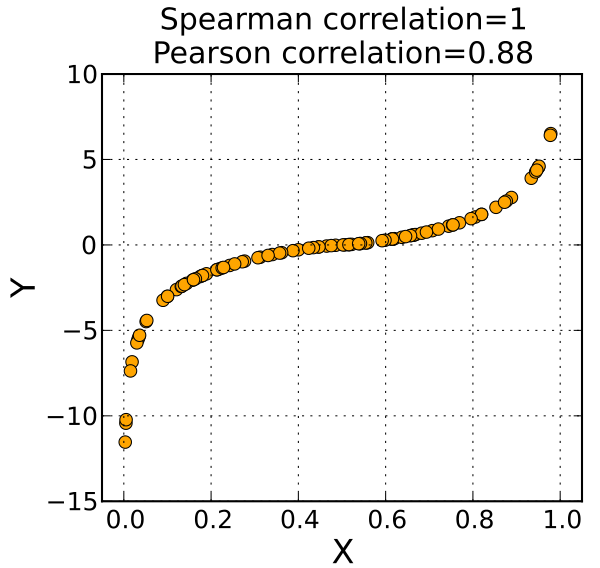
\includegraphics[width=0.475\textwidth]{P2023.AIBCCSS.InferenceAndLogisticRegression/600px-Spearman_fig1.png}
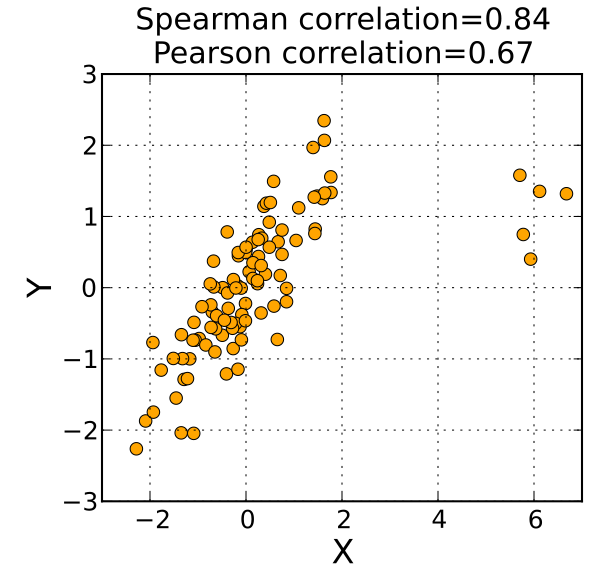
\includegraphics[width=0.475\textwidth]{P2023.AIBCCSS.InferenceAndLogisticRegression/600px-Spearman_fig3.png}

\end{center} 

\textit{\tiny
\vspace{-\baselineskip}
Source with modifications: \url{https://en.wikipedia.org/wiki/Spearman\%27s_rank_correlation_coefficient}}

\end{frame}

\begin{frame}
{\centerline{$r$ and $r_S$ (2/2)}}

\begin{center}
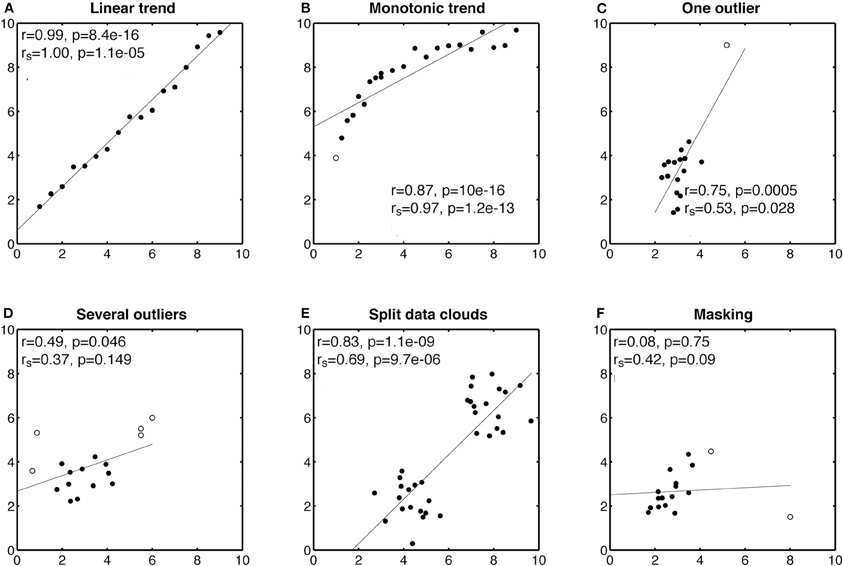
\includegraphics[width=0.7\textwidth]{P2023.AIBCCSS.InferenceAndLogisticRegression/Examples-of-Pearson-and-Spearman-correlations-In-each-subplot-r-is-Pearson-correlation.jpeg}
\end{center} 

\textit{\tiny
\vspace{-\baselineskip}
Source with modifications: \url{https://www.researchgate.net/figure/Examples-of-Pearson-and-Spearman-correlations-In-each-subplot-r-is-Pearson-correlation_fig7_224915794}}

\end{frame}

\begin{frame}
{\centerline{Notes about  $r_S$}}
\begin{itemize}
   \item If two identical values are assigned their fractional rank
   \begin{itemize}
   \item So if we have 20, 20, 30, 35, 36, then their ranks should be 1.5 (the average between 1 and 2), 1.5, 3, 4, 5 respectively
\end{itemize}
   \item Taking into account that we are dealing with integer ranks, we can simplify the formula as follows if all values are different:
   $$ r_{s}={1-{\frac {6\sum d_{i}^{2}}{n(n^{2}-1)}}}$$
   \begin{itemize}
   \item where $n$ is the number of observations and each $d_i$ is equal to the difference in rank between $X_i$ and $Y_i$:
   $$d_i = Rk_{X_i} - Rk_{Y_i}$$
\end{itemize}
\end{itemize}

\textit{\tiny
\vspace{-\baselineskip}
Source with modifications: \url{https://en.wikipedia.org/wiki/Spearman\%27s_rank_correlation_coefficient}}

\end{frame}

\begin{frame}
{\centerline{Significance of $r_S$ (1/3)}}

\begin{itemize}
    \item Being based on ordinals and non assuming anything on the distribution of the underlying populations, the computation of the significance of $r_S$ is based on permutations
    \item This belong to the family of permutation tests
    \begin{itemize}
    \item A permutation test (or exact test) is a type of statistical significance test in which the distribution of the test statistic under the null hypothesis is obtained by calculating all possible values of the test statistic under rearrangements of the labels on the observed data points
    \end{itemize}
    \item In our case, since I have sequence of ordinals, we can consider all possible pairs of mutual relationships and, based on this, determine if the monotonic relationship that we have obtained is significantly different from a random order
    
\end{itemize}

\textit{\tiny
\vspace{-\baselineskip}
Source with modifications: \url{https://en.wikipedia.org/wiki/Resampling_(statistics)\#Permutation_tests}}
\end{frame}

\begin{frame}
{\centerline{Significance of $r_S$ (2/3)}}

\begin{itemize}
    \item Consider as an example the dataset $\{(X_i,Y_i)\} = \{(10,2), (15, 0), (20, 4), (21,50)\}$
    \item Does it have a significant positive correlation?
    \item We need to assign ranks the elements, leading to $\{(Rk_{X_i},Rk_{Y_i})\} = \{(1,2), (2, 1), (3, 3), (4,4)\}$
    \item This leads to $r_S = 0.8$
    \item To compute the significance, I determine the number of times the comparison $Rk_{Y_i} \leq Rk_{Y_j}$ are true when $i<j$
    \item These are sequences of Bernoulli trials $\ldots$
    
\end{itemize}

\textit{\tiny
\vspace{-\baselineskip}
Source with modifications: \url{https://en.wikipedia.org/wiki/Resampling_(statistics)\#Permutation_tests}}
\end{frame}

\begin{frame}
{\centerline{Significance of $r_S$ (3/3)}}

\begin{itemize}
    \item It is possible to test for significance also using:
        $$w=r{\sqrt {\frac {n-2}{1-r^{2}}}}$$
    \item $w$ follows a t distribution
        $$w \sim t$$
\end{itemize}

\textit{\tiny
\vspace{-\baselineskip}
Source with modifications: \url{https://en.wikipedia.org/wiki/Spearman\%27s_rank_correlation_coefficient}}
\end{frame}


\begin{frame}
{\centerline{Kendall's $\tau$ (1/2)}}
An alternative non parametric correlation coefficient is the Kendall's $\tau$
\begin{itemize}
   \item Let's have two sets $X = \{X_i\}$ and $Y= \{Y_i\}$ of the same size $n$ where $(\forall i) X_i,Y_i \in \text{ordinal scale}$
   \item Let's consider a set of pairs $P_{X,Y} = \{(X_i,Y_i)\}$ 
   \item Let's assume that the two sets $X$ and $Y$ do not contain duplicates
   \item Let's define
   \begin{itemize}
    \item a concordant pair, a pair of pairs $(X_i,Y_i)$ and $(X_j,Y_j)$, with $i\neq j$ where either ($X_i > X_j$ and $Y_i > Y_j$) or ($X_i < X_j$ and $Y_i < Y_j$)
    \item a discordant pair, a pair of pairs $(X_i,Y_i)$ and $(X_j,Y_j)$, with $i\neq j$ where either ($X_i > X_j$ and $Y_i < Y_j$) or ($X_i > X_j$ and $Y_i < Y_j$)
\end{itemize}

\end{itemize}

\textit{\tiny
\vspace{-\baselineskip}
Source with modifications: \url{https://en.wikipedia.org/wiki/Kendall_rank_correlation_coefficient}}
\end{frame}

\begin{frame}
{\centerline{Kendall's $\tau$ (2/2)}}
\begin{itemize}
\item We can define the Kendall's $\tau$ as:
$$\tau ={\frac {({\text{\# concordant pairs}})-({\text{\# discordant pairs}})}{n(n-1)/2}}$$

\end{itemize}

\textit{\tiny
\vspace{-\baselineskip}
Source with modifications: \url{https://en.wikipedia.org/wiki/Kendall_rank_correlation_coefficient}}
\end{frame}

\begin{frame}
{\centerline{Part 3}}

\begin{center}
\Huge Logistic regression
\end{center}
\end{frame}


\begin{frame}
{\centerline{Outline}}
\begin{itemize}
\item Likelihood function, definition
\item Maximum likelihood
\item Log likelihood
\item Logistic regression
\end{itemize}

\vspace*{2cm}
Some slides are take from: \url{https://www.cs.ox.ac.uk/people/nando.defreitas/}
\end{frame}


%----------------------------------------------------------------------------------------
%------------------------------------------------
\begin{frame}
{\centerline{Likelihood function }}
Let $X_1,X_2,...,X_n$ denote a random sample from p.d.f.
$$X_i \sim f_{\theta}(x),$$
where $\theta$ represents one ore more unknown parameters of the distribution.

The joint p.d.f. of $X_1, X_2, ..., X_n$ is $f_{\theta}(x_1),f_{\theta}(x_2),...,f_{\theta}(x_n)$.

If we consider this joint p.d.f. as a function of $\theta$ it is called \textit{likelihood function} of a random sample:
$$L_{x_1,x_2,...,x_n}(\theta)=f_{\theta}(x_1),f_{\theta}(x_2),...,f_{\theta}(x_n).$$
\end{frame}

\begin{frame}
{\centerline{Maximum likelihood (1/2)}}
Let's consider an estimator of $\theta$:
$$\hat{\theta} = u(X_1,X_2,...,X_n).$$

If for every possible $\theta$ $L_{x_1,x_2,...,x_n}(\hat{\theta})$ is at least as great as $L_{x_1,x_2,...,x_n}(\theta)$ then $\hat{\theta}$ is called \textit{maximum likelihood estimator}.

Finally:
$$\hat{\theta} = \argmax\limits_{\theta}(L_{x_1,x_2,...,x_n}(\theta))$$

\end{frame}

\begin{frame}
{\centerline{Maximum loglikelihood (2/2)}}
Note that, since the likelihood function $L_{x_1,x_2,...,x_n}(\theta)$ and its logarithm $ln(L_{x_1,x_2,...,x_n}(\theta))$, are maximized for the same value $\theta$, either likelihood or its logarithm can be used to find maximum likelihood estimator:
$$\hat{\theta} = \argmax\limits_{\theta}(ln(L_{x_1,x_2,...,x_n}(\theta)))$$
\end{frame}

\begin{frame}
{\centerline{The concept of regression}}

Regressions can be of multiple types, so far we have analysed the so called OLS regression:
\begin{itemize}
\item quadratic cost function of the kind $\sum_i (\hat{y}_i - y_i)^2$
\item linear model of the kind $\hat{y} =  \mathbf{A} \mathbf{x} + \mathbf{\eta}$
\end{itemize}

\vspace*{1cm}
What if:
\begin{itemize}
\item we use a different objective function, or
\item we use a different model
\end{itemize}
\centerline{\textcolor{red}{\Huge \bf ?}}
\vspace*{1cm}
\textit{Remember that model is called ``the \textcolor{red}{mean} function'' and its inverse ``the \textcolor{red}{link} function.''}
\end{frame}

\begin{frame}
{\centerline{Posing a different problem}}
Let's suppose to have:
\begin{itemize}
\item three iid random variables $y_i$ with $ i \in [1 \ldots 3]$
\item with the same partially unknown pdf, that is
\item ($\forall i$) $y_i \thicksim N(\theta,1)$
\item $\theta$ to be determined.
\end{itemize}

We want to determine the value of $\theta$ that maximizes the probability of obtaining $y_1$ and $y_2$ and $y_3$.\\

\vspace*{0.5cm}
In other terms our objective function is the probability of occurrence of $y_1$ and $y_2$ and $y_3$.

\vspace*{0.5cm}
We are looking for a maximum likelihood estimator!

\end{frame}

\begin{frame}
{\centerline{Computing the highest probability}}
Our objective function is therefore:
$$P(y_1, y_2, y_3 | \theta) = P(y_1 | \theta) \times P(y_2 | \theta) \times P(y_3 | \theta)$$

We can rewrite this problem as:

$$ \max_{\theta}(\prod_{i=1}^3 P(y_i | \theta)) $$
%\textcolor{blue}{careful! since $\theta$ is not a random variable, $P(y_i | \theta))$ =?}
\vspace*{0.2cm}

Note that since $\theta$ is a \textit{crisp} value:
\centerline{
$ y_i \thicksim N(\theta,1) = $ a shift of $\theta$ of $N(0,1) $}


\end{frame}

\begin{frame}
{\centerline{Using concrete numbers (1/2)}}
Let us assume that:
\begin{itemize}
\item $y_1 = 1$
\item $y_2 = 0.5$
\item $y_3 = 1.5$
\end{itemize}
Remember that $N(\theta,\sigma) = \dfrac 1 {\sigma \sqrt{2 \pi} } \, e^{-\dfrac { \left({y - \theta}\right)^2} {2 \sigma^2} }$\\
\vspace{0.5cm}

Therefore, we want to maximize:\\
$ \prod_{i=1}^3 P(y_i | \theta) = \prod_{i=1}^3 \dfrac 1 {\sqrt{2 \pi} } \, e^{-\dfrac { \left({y_i - \theta}\right)^2} {2} } = $\\
\vspace{0.5cm}

$= \dfrac 1 {\sqrt{2 \pi} } \, e^{-\dfrac { \left({1 - \theta}\right)^2} {2} } \times  \dfrac 1 {\sqrt{2 \pi} } \, e^{-\dfrac { \left({0.5 - \theta}\right)^2} {2} } \times  \dfrac 1 {\sqrt{2 \pi} } \, e^{-\dfrac { \left({1.5 - \theta}\right)^2} {2} }$

\end{frame}

\begin{frame}
{\centerline{Using concrete numbers (2/2)}}

This is like maximizing:
\textcolor{blue}{
$$e^{-\dfrac { \left({1 - \theta}\right)^2} {2} } \times e^{-\dfrac { \left({0.5 - \theta}\right)^2} {2} } \times e^{-\dfrac { \left({1.5 - \theta}\right)^2} {2} } = $$
}\textcolor{cyan}{
$$ = e^{-\dfrac { \left({1 - \theta}\right)^2} {2} -\dfrac { \left({0.5 - \theta}\right)^2} {2} -\dfrac { \left({1.5 - \theta}\right)^2} {2}} = $$
}\textcolor{red}{
$$ = e^{-\dfrac { ({1 - \theta})^2 + ({0.5 - \theta})^2 + ({1.5 - \theta})^2 } {2} } = e^{-\dfrac { 3.5 - 6 \theta + 3 \theta ^2 } {2} } $$
}
This is like minimizing $ g(\theta) = 3.5 - 6 \theta + 3 \theta ^2 $.
$$\frac{d g(\theta)}{d \theta} = \frac{d 3.5 - 6 \theta + 3 \theta ^2}{d \theta} = -6 + 6 \theta$$
Which becomes 0 for $\theta = 1$

\end{frame}

\begin{frame}
{\centerline{What we have discovered }}
Our solution is therefore $\theta = 1$ and the desired pdf is $N(1,1)$. But ... 
$$mean(1, 0,5, 1.5) = 1$$

\vspace*{3.5cm}
We can try to generalize it...

\end{frame}

\begin{frame}
{\centerline{Generalizing ... }}

Let's suppose to have:
\begin{itemize}
\item $n$ iid random variables $y_i$ with $ i \in [1 \ldots n]$
\item with the same partially unknown pdf, that is
\item ($\forall i$) $y_i \thicksim N(\theta,\sigma)$
\item $\theta$ and $\sigma$ to be determined.
\end{itemize}

We want to determine the value of $\theta$ that maximizes the probability of obtaining ($\forall i$) $y_i$.\\

\vspace*{0.5cm}
In other terms our objective is to maximize the probability of occurrence of all $y_i$, that is a maximum likelihood estimation.

\vspace*{0.5cm}
Typically, we would perform a least square estimation, and we know that optimal least square estimator is the Gaussian centered in the average of the points, with their standard deviation.
\end{frame}




\begin{frame}
{\centerline{Maximum likelihood estimator (again) }}
Let' look for a maximum likelihood estimator!
$$ \max_{\sigma, \theta}(\prod_{i=1}^n P(y_i | \sigma, \theta)) = \max_{\sigma, \theta}(\prod_{i=1}^n P(y_i | \sigma, \theta)) =  \max_{\sigma, \theta}(\prod_{i=1}^n \dfrac 1 {\sigma \sqrt{2 \pi} } \, e^{-\dfrac { ({y_i - \theta})^2} {2 \sigma^2} })=$$

$$ = \max_{\sigma, \theta} \big((\dfrac 1 {\sigma \sqrt{2 \pi} } )^{n} \prod_{i=1}^n  e^{-\dfrac { ({y_i - \theta})^2} {2 \sigma^2} }\big))=
\max_{\sigma, \theta} \big((\dfrac 1 {\sigma \sqrt{2 \pi} } )^{n} e^{- \sum_{i=1}^n  \dfrac { ({y_i - \theta})^2} {2 \sigma^2} }) = $$

$$  =
\max_{\sigma, \theta} \big((\dfrac 1 {\sigma \sqrt{2 \pi} } )^{n} e^{-   \dfrac { 1 } {2 \sigma^2} \sum_{i=1}^n  ({y_i - \theta})^2} ) $$

At this point we can take the log of the expression, knowing that the log function is differentiable and monotonically increasing on all $\mathbb{R}$.

\end{frame}


\begin{frame}
{\centerline{Computing the ml estimator }}

$$log\big((\dfrac 1 {\sigma \sqrt{2 \pi} } )^{n} e^{-   \dfrac { 1 } {2 \sigma^2} \sum_{i=1}^n  ({y_i - \theta})^2} ) =$$

$$= n \times log (\dfrac 1 {\sigma \sqrt{2 \pi} }) + log(e^{ - \dfrac { 1 } {2 \sigma^2} \sum_{i=1}^n  ({y_i - \theta})^2}) =$$

$$= n \times log (\dfrac 1 {\sigma \sqrt{2 \pi} }) - \dfrac { 1 } {2 \sigma^2} \times \sum_{i=1}^n  ({y_i - \theta})^2 $$

Taking the partial derivative over $\theta$ we obtain: 

$$\frac{\partial \Big(n \times log (\dfrac 1 {\sigma \sqrt{2 \pi} }) - \dfrac { 1 } {2 \sigma^2} \times \sum_{i=1}^n  ({y_i - \theta})^2 \Big)}{\partial \theta} = $$


\end{frame}

\begin{frame}
{\centerline{Computing the ml estimator - $\theta$}}

$$ = - \frac{\partial \Big( \dfrac { 1 } {2 \sigma^2} \times \sum_{i=1}^n  ({y_i - \theta})^2 \Big)}{\partial \theta} = - \dfrac { 1 } {\sigma^2} \times \Big( \sum_{i=1}^n  ({y_i - \theta}) \Big) $$
And equating it to 0:
$$ - \dfrac { 1 } {\sigma^2} \times \Big( \sum_{i=1}^n  ({y_i - \theta}) \Big) = 0 ~\textcolor{red}{\Rightarrow}~
 \sum_{i=1}^n y_i = n \times \theta 
~\textcolor{red}{\Rightarrow}~
 \theta = \frac {\sum_{i=1}^n y_i} n  $$
 
\textcolor{red}{\bf Oh!} $\theta$ is the average of the observed $y_i$!

\end{frame}

\begin{frame}
{\centerline{Computing the ml estimator - $\sigma$ (1/2)}}
\textcolor{cyan}{
$$\frac{\partial \Big(n \times log (\dfrac 1 {\sigma \sqrt{2 \pi} }) - \dfrac { 1 } {2 \sigma^2} \times \sum_{i=1}^n  ({y_i - \theta})^2 \Big)}{\partial \sigma} = $$
}\textcolor{blue}{
$$ = \frac{\partial\Big( n \times log (\dfrac 1 {\sigma \sqrt{2 \pi} })\Big) }{\partial \sigma} - \frac{\partial \Big( \dfrac { 1 } {2 \sigma^2} \times \sum_{i=1}^n  ({y_i - \theta})^2 \Big)}{\partial \sigma} = $$
}\textcolor{red}{
$$  = - \frac n {\sigma} + \frac 1 {\sigma^3} \times \sum_{i=1}^n  ({y_i - \theta})^2$$
}
And equating it to 0:

$$ 
- \frac n {\sigma} + \frac 1 {\sigma^3} \times \sum_{i=1}^n  ({y_i - \theta})^2 = 0 
~\textcolor{red}{\Rightarrow}~
 \Big(\sum_{i=1}^n  ({y_i - \theta})^2 \Big) \times  \frac 1 {\sigma^3} = \frac n {\sigma} 
$$

\end{frame}

\begin{frame}
{\centerline{Computing the ml estimator - $\sigma$ (2/2)}}

Assuming $\sigma \ne 0$: 
$$ 
~\textcolor{red}{\Rightarrow}~
 \Big(\sum_{i=1}^n  ({y_i - \theta})^2 \Big) = n \times \sigma^2 
 ~\textcolor{red}{\Rightarrow}~
$$
But we know $\theta = \overline{y_i}$, therefore:
$$
~\textcolor{red}{\Rightarrow}~
 \sigma^2 = {\frac 1 n} \times \Big(\sum_{i=1}^n  ({y_i - \overline{y_i}})^2 \Big) 
 $$
 
\textcolor{red}{\bf Oh!} $\sigma$ is the standard deviation of the observed $y_i$!

\end{frame}

\begin{frame}
{\centerline{What we have found}}

We have determined that the maximum likelihood estimator for a sequence of points assumed to be distributed normally is formed by a normal distribution with:
\begin{itemize}
\item average equal to the average of the sample,
\item standard deviation equal to the standard derivation of the sample.
\end{itemize}

This coincides with the best quadratic estimator!
\vspace{1cm}

We now move forward considering the maximum likelihood estimator for a regression line, meaning, what happens if now we want to model an interdependencies using as objective function the maximum likelihood.

\end{frame}

\begin{frame}
{\centerline{Ml linear regression - HPs}}

Let's suppose to have:
\begin{itemize}
\item $n \times m$ values $x_{i,j}$ with $ i \in [1 \ldots n]$, $ j \in [1 \ldots m]$ represented in short by a matrix $\boldsymbol{X}$ or a vector $\mathbf{x_i}$, $n>m$ \textit{(why?)}
\item $n$ iid random variables $y_i$ with $ i \in [1 \ldots n]$ represented in short by a vector $\boldsymbol{y}$
\item a linear relationships $\boldsymbol{\theta}$ between $\boldsymbol{X}$  and $\boldsymbol{y}$, \textit{that is, we use the usual \textcolor{red}{link / mean} functions}
\item each $y_i$ distributed normally with mean $\boldsymbol{x_i^T \theta}$ and standard deviation $\sigma$ (the same $\sigma$ for all $y_i$), that is 
\item ($\forall i$) $y_i \thicksim N(\boldsymbol{x_i^T \theta},\sigma)$
\item $\boldsymbol{\theta}$ and $\sigma$ to be determined.
\end{itemize}
\end{frame}

\begin{frame}
{\centerline{Ml linear regression - goals}}

We want to determine the value of $\boldsymbol{\theta}$ and $\sigma$ that maximizes the probability of obtaining ($\forall i$) $y_i$, that is:

$$ \max_{\theta, \sigma}( P(\mathbf{y} | \boldsymbol{X}, \boldsymbol{\theta}, \sigma)) = \max_{\boldsymbol{\theta}, \sigma}(\prod_{i=1}^n P(y_i | \boldsymbol{x_i}, \boldsymbol{\theta}, \sigma)) $$


\vspace*{0.5cm}
In other terms, our objective function is the conditional probability of occurrence of all $y_i$.


\end{frame}

\begin{frame}
{\centerline{Computing the optimal $\theta$ (1/3)}}
We can express for simplicity our equation in vectorial form:
$$\max_{\sigma, \boldsymbol{\theta}}\left ( \left (\dfrac 1 {\sigma \sqrt{2 \pi} } \right)^n \, e^{-\dfrac { (\boldsymbol{y} - \boldsymbol{X\theta})^T (\boldsymbol{y} - \boldsymbol{X\theta})} {2 \sigma^2} }\right)$$

As mentioned, this is equivalent to maximizing the log:

$$\max_{\sigma, \boldsymbol{\theta}} \left( log \left (\left (\dfrac 1 {\sigma \sqrt{2 \pi} } \right )^n \, e^{-\dfrac { (\boldsymbol{y} - \boldsymbol{X\theta})^T (\boldsymbol{y} - \boldsymbol{X\theta})} {2 \sigma^2} }\right) \right )$$

Which becomes:
$$\max_{\sigma, \boldsymbol{\theta}} \left( n \times log \left (\dfrac 1 {\sigma \sqrt{2 \pi} } \right ) + log \left( \, e^{-\dfrac { (\boldsymbol{y} - \boldsymbol{X\theta})^T (\boldsymbol{y} - \boldsymbol{X\theta})} {2 \sigma^2} }\right) \right )$$

\end{frame}

\begin{frame}
{\centerline{Computing the optimal $\theta$ (2/3)}}

$$\max_{\sigma, \boldsymbol{\theta}} \left( n \times log \left (\dfrac 1 {\sqrt{2 \pi} } \right ) + n \times log \left (\dfrac 1 {\sigma } \right ) -\dfrac { (\boldsymbol{y} - \boldsymbol{X\theta})^T (\boldsymbol{y} - \boldsymbol{X\theta})} {2 \sigma^2} \right )$$

And now we take the partial derivative over $\boldsymbol{\theta}$:

$$\frac{\partial \left( n \times log \left (\dfrac 1 {\sqrt{2 \pi} } \right ) + n \times log \left (\dfrac 1 {\sigma } \right ) -\dfrac { (\boldsymbol{y} - \boldsymbol{X\theta})^T (\boldsymbol{y} - \boldsymbol{X\theta})} {2 \sigma^2} \right )} {\partial \boldsymbol{\theta}} = $$

$$= - \frac 1 {2 \sigma^2} \frac{\partial \left( { (\boldsymbol{y} - \boldsymbol{X\theta})^T (\boldsymbol{y} - \boldsymbol{X\theta})} \right )} {\partial \boldsymbol{\theta}} =  - \frac 1 {\sigma^2}  { (\boldsymbol{y} - \boldsymbol{X\theta})}  $$
And equating it to 0 we obtain:
$$ - \frac 1 {\sigma^2}  { (\boldsymbol{y} - \boldsymbol{X\theta})} = 0
~~~\textcolor{red}{\Rightarrow}~~~
\boldsymbol{y} = \boldsymbol{X\theta}
$$



\end{frame}

\begin{frame}
{\centerline{Computing the optimal $\theta$ (3/3)}}

If $\boldsymbol{X}$ were square, then the solution would be:
$$ \boldsymbol{\theta} = \boldsymbol{X^{-1}y}$$

But, as we said, $n > m$, therefore the solution is given by:

$$ \boldsymbol{\theta} = \boldsymbol{{(X^{T}X})^{-1}X^{T}y}$$

\vspace{2cm}

What a surprise, isn't it?
\end{frame}

\begin{frame}
{\centerline{Computing the optimal $\sigma$ }}
Starting from: 
$$\max_{\sigma, \boldsymbol{\theta}} \left( n \times log \left (\dfrac 1 {\sqrt{2 \pi} } \right ) + n \times log \left (\dfrac 1 {\sigma } \right ) -\dfrac { (\boldsymbol{y} - \boldsymbol{X\theta})^T (\boldsymbol{y} - \boldsymbol{X\theta})} {2 \sigma^2} \right )$$

And now we take the partial derivative over $\sigma$:

$$\frac{\partial \left( n \times log \left (\dfrac 1 {\sqrt{2 \pi} } \right ) + n \times log \left (\dfrac 1 {\sigma } \right ) -\dfrac { (\boldsymbol{y} - \boldsymbol{X\theta})^T (\boldsymbol{y} - \boldsymbol{X\theta})} {2 \sigma^2} \right )} {\partial \sigma} = $$

$$= - \dfrac n {\sigma } +  \dfrac { (\boldsymbol{y} - \boldsymbol{X\theta})^T (\boldsymbol{y} - \boldsymbol{X\theta})} { \sigma^3 } $$
And equating it to 0, assuming as usual $\sigma \ne 0$ we obtain:
$$ \sigma^2 = \dfrac { (\boldsymbol{y} - \boldsymbol{X\theta})^T (\boldsymbol{y} - \boldsymbol{X\theta})} { n }
$$


\end{frame}

\begin{frame}
{\centerline{Maximum likelihood estimator - properties}}
\underline{Claim 1:} The maximum likelihood estimator of a Gaussian distribution over a set of points coincides with the OLS estimator.\\
\underline{Proof:} See above.\\
\underline{QED}

\vspace{2cm}
\underline{Claim 2:} The maximum likelihood linear regression coincides with the OLS linear regression.\\
\underline{Proof:} See above.\\
\underline{QED}


\end{frame}


\begin{frame}
{\centerline{Bernoulli and maximum likelihood}}

The pdf of a Bernulli distribution can be represented in terms of conditional probability as:
$$ P(x | \theta) = \theta^x (1-\theta)^{(1-x)} $$
where clearly $x$ can only be 0 or 1.
\newline

We can now introduce the concept of entropy, already hinted in class. Entropy represents the level of uncertainty of a variable.


\end{frame}

\begin{frame}
{\centerline{Entropy (and Bernulli and ml)}}

\underline{Definition (Entropy):} Given a random vectorial variable $\boldmath{x}$ of $n$ components and a parameter $\theta$, we define entropy of $\boldmath{x}$, $H(\boldmath{x})$ as:
$$H(\boldmath{x}) = \sum_{i=1}^{n} p(x_i|\theta) \times log (p(x_i|\theta)) $$

We notice that for a Bernulli distribution:
$$ H(\boldmath{x}) = (1-\theta) log (1-\theta) + \theta log(\theta)$$

Indeed, as $\theta$ tends to 0 or to 1 the uncertainty tends to 0, since the likely value of $\boldmath{x}$ tend to be 0 or 1 respectively.

\end{frame}

\begin{frame}
{\centerline{From B\&B plus ml to LR}}
We are now ready to move to study a radically different form or regression, the so-called logistic regression.
\newline

Our goal is to have a regression that not only represents a relationship between two variables, but is also possible to capture a prediction of probability.
\newline

However, the value of a probability is from 0 to 1, so we need a ``good'' function that can translate any value in such range.
\newline

We use often as such function the so-called ``sigmoid function.'' To introduce the sigmoid we start with the definition of a ``logistic function.''

\end{frame}

\begin{frame}
{\centerline{Logistic}}
\underline{Definition (Logistic function):} Given $L, x_0 \in \mathbb{R}$, $k \in \mathbb{R}^+$ a
logistic function $f(x)$ is defined as: 
$$ f(x) = \dfrac{L}{1+e^{-k(x-x_0)}}$$
\underline{Properties (of the logistic function:)}
\begin{itemize}
\item the domain is all $\mathbb{R}$
\item the range is $[0 \ldots L]$ if $L$ is positive and $[L \ldots 0]$ if $L$ is negative
\item $f(x)$ is continuous, monotonically increasing, and differentiable  over all its domain
\item $f(x)$ is symmetric over $x_0$
\item $k$ is the rate of growth of $f(x)$ and for $k \to +\infty$ $f(x)$ tends to become the step function in $x_0$
\end{itemize}

\end{frame}

\begin{frame}
{\centerline{Sigmoid}}
\underline{Definition (Sigmoid):} Given $k \in \mathbb{R}^+$, a
sigmoid function $sigm(x)$ is defined as a logistic function with $L = 1$ and $x_0 = 0$: 
$$ sigm(x) = \dfrac{1}{1+e^{-kx}}$$
\underline{Properties (of the sigmoid function):}
\begin{itemize}
\item the domain is all $\mathbb{R}$
\item the range is $[0 \ldots 1]$ 
\item $sigm(x)$ is continuous, monotonically increasing, and differentiable  over all its domain
\item $sigm(x)$ is symmetric over $0$
\item $k$ is the rate of growth of $sigm(x)$ and for $k \to +\infty$ $sigm(x)$ tends to become the step function
\end{itemize}

\end{frame}

\begin{frame}
{\centerline{Toward a logistic regression (1/2)}}

Suppose that we want to determine if a given event is going to happen based on a series of $n$ predictors $x_1 \ldots x_n$. We can model the probability of occurrence of the event with a random variable $y$.
\newline

It is as if we have a sequence of flipping of coins each with different values of the possible variables that affect the result, for instance the intensity of the flipping, the temperature, the wind, etc.
\newline

Based on such set we want to  predict what will be the result of the next flipping, given a set of values assigned to the covariates.
\newline

Our question is what is:
\begin{center}
P(Head $|$ strong toss, strong wind, 60 degrees)\\

{\Huge \textcolor{red}{\bf ?}}
\end{center}



\end{frame}

\begin{frame}
{\centerline{Toward a logistic regression (2/2)}}
Let's try to build a regression line.
\newline

As we mentioned, any time we compute a regression we need to determine:
\begin{itemize}
\item the function to use as a model, and in this case a linear function would not be suitable, since probabilities range from 0 to 1, for this reason we select a \textcolor{red}{sigmoid function};
\item the objective function, and in this case the least square would be inappropriate because it is not a proper metrics space, so we opt for maximizing the conditional probability, that is, we aim at a \textcolor{red}{maximum likelihood} estimation.
\end{itemize}



\end{frame}

\begin{frame}
{\centerline{{\centerline{Logistic regression - HPs}}}}
Let 
\begin{itemize}
\item $(y_i,\boldmath{x_i})$  be a collection of pairs with:
\begin{itemize}
\item $i \in [1 \ldots n]$
\item $y_i \in \{0,1\}$
\item $\boldmath{x_i} \in \mathbb{R}^{m}$
\item $n > m$
\end{itemize}
\item assume that the $y_i$ are iid random variables
\item consider as target \textcolor{red}{mean} function the sigmoid
\item consider as optimality criteria the maximum likelihood
\end{itemize}

\end{frame}

\begin{frame}
{\centerline{{\centerline{Logistic regression - goals}}}}

We want to determine the values of the parameters that maximize the probability of obtaining ($\forall i$) $y_i$, that is:

$$ \max_{\text{\bf \it Parameters}}( P(\mathbf{y} | \boldsymbol{X}, \text{\bf \it Parameters}) = \max_{\boldsymbol{\theta}}(\prod_{i=1}^n P(y_i | \boldsymbol{x_i}, \text{\bf \it Parameters})) $$


\vspace*{0.5cm}
In other terms, our objective function is the conditional probability of occurrence of all $y_i$.
\vspace*{0.5cm}

Given our link/mean: 
$$ \max_{\theta}( P(\mathbf{y} | \boldsymbol{X}, \boldsymbol{\theta})) = \max_{\boldsymbol{\theta}}(\prod_{i=1}^n P(y_i | sigm(\boldsymbol{x_i}^{T} \boldsymbol{\theta})) $$

\end{frame}

\begin{frame}
{\centerline{{\centerline{Logistic regression - structure}}}}

Since the pdf of a Bernulli distribution is:
$$ P(z | k) = k^z (1-k)^{(1-z)} $$
For us the probability k of each event is ``approximated'' by the sigmoid function (our mean function):

$$ \boldsymbol{k} = \dfrac{1}{1+e^{-\boldsymbol{x_i}^{T} \boldsymbol{\theta}}}$$

And this lead us to

$$ P(y_i | \boldsymbol{x_i}, \boldsymbol{\theta}) = \left ( \dfrac{1}{1+e^{-\boldsymbol{x_i}^{T} \boldsymbol{\theta}}} \right )^{y_i} \times \left (1 - \dfrac{1}{1+e^{-\boldsymbol{x_i}^{T} \boldsymbol{\theta}}} \right )^{1-y_i}  $$


\end{frame}

\begin{frame}
{\centerline{{\centerline{Logistic regression - the problem }}}}

Our problem has therefore the form of:
$$ \max_{\theta}( P(\mathbf{y} | \boldsymbol{X}, \boldsymbol{\theta})) =  \max_{\boldsymbol{\theta}} \prod_{i=1}^n \left ( \dfrac{1}{1+e^{-\boldsymbol{x_i}^{T} \boldsymbol{\theta}}} \right )^{y_i} \times \left ( 1-\dfrac{1}{1+e^{-\boldsymbol{x_i}^{T} \boldsymbol{\theta}}} \right )^{1-y_i} $$

\textit{It is like finding an n-dimensional hyperplane dividing the n-dimensional hyperspace in 2 parts, those leading to y being 0 and those leading to y being 1.}

\vspace*{3cm}

\end{frame}


\begin{frame}
{\centerline{{\centerline{Logistic regression - solution (1/3)}}}}
Since the log function is continuous, differentiable and monotonically increasing in all ${\mathbb{R}^+}$, our problem is equivalent to:
$$ \max_{\boldsymbol{\theta}} \left ( log \left ( \prod_{i=1}^n \left ( \dfrac{1}{1+e^{-\boldsymbol{x_i}^{T} \boldsymbol{\theta}}} \right )^{y_i} \times \left (1 - \dfrac{1}{1+e^{-\boldsymbol{x_i}^{T} \boldsymbol{\theta}}} \right )^{1-y_i} \right ) \right )$$

And, given the property of logs, this is like maximizing:
\textcolor{blue}{
$$ log \left ( \prod_{i=1}^n \left ( \dfrac{1}{1+e^{-\boldsymbol{x_i}^{T} \boldsymbol{\theta}}} \right )^{y_i}  \right ) + log \left (  \prod_{i=1}^n \left (1 - \dfrac{1}{1+e^{-\boldsymbol{x_i}^{T} \boldsymbol{\theta}}} \right )^{1-y_i} \right ) = $$
}\textcolor{red}{
$$ = \sum_{i=1}^n log \left ( \dfrac{1}{1+e^{-\boldsymbol{x_i}^{T} \boldsymbol{\theta}}} \right )^{y_i}  + \sum_{i=1}^n log \left (1 - \dfrac{1}{1+e^{-\boldsymbol{x_i}^{T} \boldsymbol{\theta}}} \right )^{1-y_i} = $$
}
\end{frame}
\begin{frame}
{\centerline{{\centerline{Logistic regression - solution (2/3)}}}}
\textcolor{gray}{
$$  = \sum_{i=1}^n y_i \times log \left ( \dfrac{1}{1+e^{-\boldsymbol{x_i}^{T} \boldsymbol{\theta}}} \right ) + \sum_{i=1}^n (1-y_i) \times log \left (1 - \dfrac{1}{1+e^{-\boldsymbol{x_i}^{T} \boldsymbol{\theta}}} \right ) = \cdots{} $$
}
A bit of logarithms...
\textcolor{blue}{
 $$log \left ( \dfrac{1}{1+e^{-\boldsymbol{x_i}^{T} \boldsymbol{\theta}}} \right ) = log (1) - log \left( 1+e^{-\boldsymbol{x_i}^{T} \boldsymbol{\theta}} \right ) = -log \left( 1+e^{-\boldsymbol{x_i}^{T} \boldsymbol{\theta}} \right )$$
 }
 
 \textcolor{cyan}{
 $$log \left ( 1 - \dfrac{1}{1+e^{-\boldsymbol{x_i}^{T} \boldsymbol{\theta}}} \right ) = log \left ( \dfrac{1 + e^{-\boldsymbol{x_i}^{T} \boldsymbol{\theta}} - 1}{1+e^{-\boldsymbol{x_i}^{T} \boldsymbol{\theta}}} \right ) = log \left ( \dfrac{e^{-\boldsymbol{x_i}^{T} \boldsymbol{\theta}}}{1+e^{-\boldsymbol{x_i}^{T} \boldsymbol{\theta}}} \right ) =$$
$$= log \left ( e^{-\boldsymbol{x_i}^{T}\boldsymbol{\theta}} \right ) - log \left( 1+e^{-\boldsymbol{x_i}^{T} \boldsymbol{\theta}} \right ) =  \boldsymbol{x_i}^{T}\boldsymbol{\theta} - log \left( 1+e^{-\boldsymbol{x_i}^{T} \boldsymbol{\theta}} \right ) = $$
 }

\end{frame}

\begin{frame}
{\centerline{{\centerline{Logistic regression - solution (3/3)}}}}

$$ = - \sum_{i=1}^n y_i \times log \left( 1+e^{-\boldsymbol{x_i}^{T} \boldsymbol{\theta}} \right ) + \sum_{i=1}^n (1-y_i) \times  \left ( \boldsymbol{x_i}^{T}\boldsymbol{\theta} - log \left( 1+e^{-\boldsymbol{x_i}^{T} \boldsymbol{\theta}} \right ) \right ) = $$
For simplicity let $w_i$ be $log \left( 1+e^{-\boldsymbol{x_i}^{T} \boldsymbol{\theta}} \right )$.
\textcolor{red}{
$$
= - \sum_{i=1}^n y_i \times w_i + \sum_{i=1}^n \boldsymbol{x_i}^{T}\boldsymbol{\theta} - \sum_{i=1}^n w_i - \sum_{i=1}^n y_i \times \boldsymbol{x_i}^{T}\boldsymbol{\theta} + \sum_{i=1}^n y_i \times w_i =
$$
}\textcolor{orange}{
$$
= \sum_{i=1}^n \boldsymbol{x_i}^{T}\boldsymbol{\theta} - \sum_{i=1}^n w_i - \sum_{i=1}^n y_i \times \boldsymbol{x_i}^{T}\boldsymbol{\theta}  =
$$
}\textcolor{blue}{
$$
= \sum_{i=1}^n (1 + y_i) \boldsymbol{x_i}^{T}\boldsymbol{\theta} - \sum_{i=1}^n w_i 
$$
}
\end{frame}

\begin{frame}
{\centerline{{\centerline{Logistic regression - comments }}}}

Let $f(\boldmath{\theta})$ be:
$$
\textcolor{red}{ \sum_{i=1}^n (1 + y_i) \boldsymbol{x_i}^{T}\boldsymbol{\theta} } - 
\textcolor{blue}{\sum_{i=1}^n log \left( 1+e^{-\boldsymbol{x_i}^{T} \boldsymbol{\theta}} \right ) }
$$
\underline{Claim:} $f(\boldmath{\theta})$ is convex.
\newline

\underline{Proof:} Omitted
\newline

\underline{Consequence:}
Optimization algorithms can easily find the maximum.


\end{frame}





\end{document}
